\documentclass[openany]{book}
%%%%% PREAMBLE
%BEGIN_FOLD
%%%%% PACKAGES
\usepackage{amsmath}
\usepackage{amssymb}
\usepackage{amsthm}
\usepackage{cabin} % section title font
\usepackage[default]{cantarell} % default font
\usepackage{capt-of}
\usepackage[shortlabels]{enumitem}
\usepackage{fancyhdr}
\usepackage{graphicx}
\usepackage{hyperref}
\usepackage[utf8]{inputenc}
\usepackage{listings}
\usepackage{mathtools}
\usepackage[framemethod=TikZ]{mdframed}
\usepackage{multirow}
\usepackage[scr]{rsfso} % power set symbol
\usepackage{tasks} % vaguely remember this being important for something...?
\usepackage{tikz} % diagrams
\usepackage{titlesec}
\usepackage{thmtools}
\usetikzlibrary{shapes.geometric}
\usepackage{varwidth}
\usepackage{verbatim} % longer comments
\usepackage{xcolor}
%%%%%

%%%%% COLOURS
\definecolor{darkgreen}{HTML}{19A514}
\definecolor{lightgreen}{HTML}{9DFF9A}
\definecolor{darkblue}{HTML}{3E5FE4}
\definecolor{lightblue}{HTML}{BCDEFF}
\definecolor{darkred}{HTML}{CC3333}
\definecolor{lightred}{HTML}{FFA9A9}
\definecolor{darkpurple}{HTML}{A933CD}
\definecolor{lightpurple}{HTML}{F0BAFF}
\definecolor{darkyellow}{HTML}{D2D22A}
\definecolor{lightyellow}{HTML}{FFFFAE}
\definecolor{darkorange}{HTML}{FF6600}
\definecolor{lightorange}{HTML}{FAC098}
\definecolor{hyperlinkblue}{HTML}{3366CC}
%%%%%

%%%%% PAGE SETUP
% basic %
\setlength\parindent{0pt} % paragraph indentation
\setlength{\parskip}{5pt} % spacing between paragraphs
\usepackage[margin=1in]{geometry} % margin size

% header/footer %
\pagestyle{fancy}
\fancyhf{}
\renewcommand{\headrulewidth}{0pt} % removing horizontal line at the top
\setlength{\headheight}{15pt}
\renewcommand{\chaptermark}[1]{\markright{#1}{}}
\renewcommand{\sectionmark}[1]{}
\fancypagestyle{contentpage}{%
	\lhead{}
	\rhead{\textit{\rightmark}}
	\cfoot{\thepage}
}
\pagestyle{contentpage}

% table of content %
\makeatletter
\newcommand\mytoc{%
	\if@twocolumn
	\@restonecoltrue\onecolumn
	\else
	\@restonecolfalse
	\fi
	\toctrue
	\chapter*{\contentsname
		\@mkboth{%
			\contentsname}{\contentsname}}\addcontentsline{toc}{chapter}{Contents}%
	\tocfalse
	\@starttoc{toc}%
	\if@restonecol\twocolumn\fi
}
\makeatother

% chapter formatting %
\newif\iftoc
\titleformat
{\chapter} % command
[display] % shape
{\cabin} % font
{} % label
{2in} % 
{
	\raggedleft
	\iftoc
	\vspace{2in}
	\else
	{\LARGE\textsc{Chapter}~{\cantarell\thechapter}} \\
	\fi
	\Huge\scshape\bfseries
}
[
\vspace{-20pt}%
\rule{\textwidth}{0.1pt}
\vspace{0.0in}
]
\titlespacing{\chapter}
{0pt}
{
	\iftoc
	-100pt+1in
	\else
	-130pt+1in
	\fi
}
{0pt}

% hyperlink formatting %
\hypersetup{
	colorlinks,    
	linkcolor=hyperlinkblue,
	urlcolor=hyperlinkblue,
	pdftitle={...},
	pdfauthor={Michael Pham},
}
%%%%%

%%%%% ENVIRONMENTS STYLES
% lstlistings
\lstset{
	tabsize=4,
	belowskip=0pt
}
% purple box %
\declaretheoremstyle[
mdframed={
	backgroundcolor=lightpurple,
	linecolor=darkpurple,
	rightline=false,
	topline=false,
	bottomline=false,
	linewidth=2pt,
	innertopmargin=8pt,
	innerbottommargin=8pt,
	innerleftmargin=8pt,
	leftmargin=-2pt,
	skipbelow=2pt,
	nobreak
},
headfont=\normalfont\bfseries\color{darkpurple}
]{purplebox}

% green box %
\declaretheoremstyle[
mdframed={
	backgroundcolor=lightgreen,
	linecolor=darkgreen,
	rightline=false,
	topline=false,
	bottomline=false,
	linewidth=2pt,
	innertopmargin=8pt,
	innerbottommargin=8pt,
	innerleftmargin=8pt,
	leftmargin=-2pt,
	skipbelow=2pt,
	nobreak
},
headfont=\normalfont\bfseries\color{darkgreen}
]{greenbox}

% yellow box %
\declaretheoremstyle[
mdframed={
	backgroundcolor=lightyellow,
	linecolor=darkyellow,
	rightline=false,
	topline=false,
	bottomline=false,
	linewidth=2pt,
	innertopmargin=8pt,
	innerbottommargin=8pt,
	innerleftmargin=8pt,
	leftmargin=-2pt,
	skipbelow=2pt,
	nobreak
},
headfont=\normalfont\bfseries\color{darkyellow}
]{yellowbox}

% blue box %
\declaretheoremstyle[
mdframed={
	backgroundcolor=lightblue,
	linecolor=darkblue,
	rightline=false,
	topline=false,
	bottomline=false,
	linewidth=2pt,
	innertopmargin=8pt,
	innerbottommargin=8pt,
	innerleftmargin=8pt,
	leftmargin=-2pt,
	skipbelow=2pt,
	nobreak
},
headfont=\normalfont\bfseries\color{darkblue}
]{bluebox}

% red box %
\declaretheoremstyle[
mdframed={
	backgroundcolor=lightred,
	linecolor=darkred,
	rightline=false,
	topline=false,
	bottomline=false,
	linewidth=2pt,
	innertopmargin=8pt,
	innerbottommargin=8pt,
	innerleftmargin=8pt,
	leftmargin=-2pt,
	skipbelow=2pt,
	nobreak
},
headfont=\normalfont\bfseries\color{darkred}
]{redbox}

% orange box %
\declaretheoremstyle[
mdframed={
	backgroundcolor=lightorange,
	linecolor=darkorange,
	rightline=false,
	topline=false,
	bottomline=false,
	linewidth=2pt,
	innertopmargin=8pt,
	innerbottommargin=8pt,
	innerleftmargin=8pt,
	leftmargin=-2pt,
	skipbelow=2pt,
	nobreak
},
headfont=\normalfont\bfseries\color{darkorange}
]{orangebox}
%%%%%

%%%%% ENVIRONMENTS
% SOLUTION ENVIRONMENT %
\newenvironment{solution}{\begin{proof}[Solution]}{\end{proof}}

% purple boxes (theorems, propositions, lemmas, and corollaries) %
\declaretheorem[style=purplebox,name=Theorem,within=chapter]{thm}
\declaretheorem[style=purplebox,name=Theorem,sibling=thm]{theorem}
\declaretheorem[style=purplebox,name=Theorem,numbered=no]{thm*, theorem*}
\declaretheorem[style=purplebox,name=Proposition,sibling=thm]{prop, proposition}
\declaretheorem[style=purplebox,name=Proposition,numbered=no]{prop*, proposition*}
\declaretheorem[style=purplebox,name=Lemma,sibling=thm]{lem, lemma}
\declaretheorem[style=purplebox,name=Lemma,numbered=no]{lem*, lemma*}
\declaretheorem[style=purplebox,name=Corollary,sibling=thm]{cor, corollary}
\declaretheorem[style=purplebox,name=Corollary,numbered=no]{cor*, corollary*}

% green boxes (definitions) %
\declaretheorem[style=greenbox,name=Definition,sibling=thm]{definition, defn}
\declaretheorem[style=greenbox,name=Definition,numbered=no]{definition*, defn*}

% red boxes (problems) %
\declaretheorem[style=redbox,name=Problem,numberwithin=chapter]{homework, hw}
\declaretheorem[style=redbox,name=Problem,numbered=no]{homework*, hw*}

% blue boxes (exercises) %
\declaretheorem[style=bluebox,name=Example,sibling=thm]{example, ex}
\declaretheorem[style=bluebox,name=Example,numbered=no]{example*, ex*}

% orange boxes (remarks) %
\declaretheorem[style=orangebox,name=Remark,sibling=thm]{remark, rmk}
\declaretheorem[style=orangebox,name=Remark,numbered=no]{remark*, rmk*}
\declaretheorem[style=orangebox,name=Observation,sibling=thm]{observation, obs}
\declaretheorem[style=orangebox,name=Observation,numbered=no]{observation*, obs*}

% yellow boxes (warnings) %
\declaretheorem[style=yellowbox,name=Warning,sibling=thm]{warn}
\declaretheorem[style=yellowbox,name=Warning,numbered=no]{warn*}
%%%%%

%%%%% PROOF FORMATTING
\renewcommand\qedsymbol{$\blacksquare$}
%%%%%

%%%%% CUSTOM COMMANDS
% basic %
\newcommand{\Mod}[1]{\ (\mathrm{mod}\ #1)}
\newcommand{\floor}[1]{\left\lfloor{#1}\right\rfloor}
\newcommand{\ceil}[1]{\left\lceil{#1}\right\rceil}
\newcommand{\norm}[1]{\left\lVert{#1}\right\rVert}

% logic %
\newcommand*\xor{\oplus}
\newcommand{\all}{\forall}
\newcommand{\bland}{\bigwedge}
\newcommand{\blor}{\bigvee}
\newcommand*{\defeq}{\coloneqq}

% matrices %
\newcommand\aug{\fboxsep=- \fboxrule\!\!\!\fbox{\strut}\!\!\!}

% sets %
\newcommand{\CC}{\mathbb{C}}
\newcommand{\NN}{\mathbb{N}}
\newcommand{\QQ}{\mathbb{Q}}
\newcommand{\RR}{\mathbb{R}}
\newcommand{\ZZ}{\mathbb{Z}}

% title %
\newcommand{\mytitle}[2]{%
	\title{#1}
	\author{Michael Pham}
	\date{#2}
	\maketitle
	\newpage
	\mytoc
	\newpage
}
%%%%%

%%%%% REDEFINING COMMANDS
\let\oldint\int
\renewcommand{\int}[2]{\oldint\limits_{#1}^{#2}}
\let\oldprod\prod
\renewcommand{\prod}[2]{\oldprod\limits_{#1}^{#2}}
\let\oldsum\sum
\renewcommand{\sum}[2]{\oldsum\limits_{#1}^{#2}}
%%%%%
%END_FOLD
%%%%%


\begin{document}
\mytitle{Notes on Discrete Mathematics}{Spring 2023}
\setcounter{chapter}{-1}
\chapter{Introduction}
\section{Introduction}

Before proceeding with the rest of the course notes, we will first review the idea of sets and mathematical notation. 

\subsection{Sets} 
\begin{defn}[Set]
	A \textbf{set} is a well defined collection of objects; these objects are referred to as elements or members of the set. They aren't restricted to being just numbers; they can be letters, people, cities, and even other sets.
\end{defn}

Sets are usually denoted by capital letters, with the elements surrounded by curly brackets. For example, let $A$ denote the set of the first five prime numbers. Then, to express this set, we can write it as the following: $A=\{2,3,5,7,11\}$. If $x$ is an element of the set $A$, we can write $x\in A$. If an element $y$ is not contained in the set of $A$, we can write $y \notin A$.

Two sets $A$ and $B$ are equal to each other if they contain the same element. Note here that the order in which the elements appear in does not matter; i.e. $\{1,2,3\}=\{1,3,2\}=\ldots$

Sometimes, more complicated sets can be defined by using a different notation. An example of this is the set of all rational numbers, $\mathbb{Q}$, which can be written as: $\{\frac{a}{b}:a,b\in\mathbb{Z}, b\neq0\}$.

\subsubsection{Cardinality} 
\begin{defn}[Cardinality]
	The size of a set is referred to as its $\textbf{cardinality}$. If $A=\{2,3,5,7,11\}$, then its cardinality, denoted as $\lvert A\rvert$, is $5$.
\end{defn}

It is possible for a set to have a cardinality of $0$; this unique set, called the $\textbf{empty set}$, is denoted by the symbol $\emptyset$.

It is also possible for a set to have an infinite number of elements. Examples of such sets includes the set of all integers, prime numbers, etc.

\newpage

\subsubsection{Subsets and Proper Subsets} 
\begin{defn}[Subset]
	If every element in $A$ is also contained in $B$, then we say that $A$ is a $\textbf{subset}$ of $B$, denoted by $A\subseteq B$.
\end{defn}

\begin{defn}[Proper Subset]
	A $\textbf{proper subset}$ is a set $A$ that is strictly contained in $B$; in other words, there's at least one element in $B$ that isn't in $A$.
\end{defn}

\begin{example}
	For example, if $B=\{2,3,5,7,11\}$, then if $A=\{2,3,5\}$ then it is a proper subset of $B$. However, if $A=\{2,3,5,7,11\}$, then it isn't a proper subset. A proper subset is denoted by $A\subset B$.
\end{example}

The following are a few basic properties of subsets:
\begin{enumerate}
	\item The empty set, denoted by $\{\}$ or $\emptyset$, is a proper subset of any non-empty set $A$: $\{\}\subset A$.
	\item The empty set is a subset of every set $B$: $\{\}\subseteq B$.
	\item Any set $C$ is a subset of itself: $C\subseteq C$.
\end{enumerate}

\subsubsection{Intersections and Unions}
\begin{defn}[Intersection]
	The $\textbf{intersection}$ of a set $A$ and $B$ are all the elements that are contained in both $A$ and $B$. This is denoted by $A\cap B$.
\end{defn}

Two sets are considered $\textbf{disjoint}$ if $A \cap B = \emptyset$.

\begin{defn}[Union]
	The $\textbf{union}$ of $A$ and $B$, denoted by $A\cup B$, are all elements in $A$, $B$, or both. 
\end{defn}

\begin{example}
	For example, let $A=\{2n:n\in\mathbb{Z}\}$ and $B=\{2n+1:n\in\mathbb{Z}\}$. In English, $A$ is the set of all even numbers, and $B$ is the set of all odd numbers. Then, for these, $A\cap B=\emptyset$ and $A\cup B=\mathbb{Z}^+$.
\end{example}

The following are properties of intersections and unions:
\begin{enumerate}
	\item $A\cup B=B\cup A$.
	\item $A\cup\emptyset = A$.
	\item $A\cap B = B\cap A$.
	\item $A\cap\emptyset=\emptyset$.
\end{enumerate}

\subsubsection{Complements}
\begin{defn}[Complement]
	The $\textbf{complement}$ of a set $A$, denoted by $A^C$ or $A'$, is the set of elements not contained in $A$.
\end{defn}

\begin{defn}[Relative Complement]
	If $A$ and $B$ are two sets, then the $\textbf{relative complement}$ of $A$ in $B$, or the $\textbf{set difference}$ between $B$ and $A$, is the set of elements in $B$ but not in $A$. This is denoted as $B-A$ or $B\backslash A=\{x\in B:x \not\in A\}$.
\end{defn}

\begin{example}
	For example, if $B=\{2,3,5,7,11\}$ and $A=\{2,3,7\}$, then $B\backslash A=\{5,11\}$. Another example is for the set of all real numbers $\mathbb{R}$ and rational numbers $\mathbb{Q}$: $\mathbb{R}\backslash\mathbb{Q}$ is the set of all irrational numbers.
\end{example}

The following are important properties of complements:
\begin{enumerate}
	\item $A\backslash A = \emptyset$.
	\item $A\backslash\emptyset = A$.
	\item $\emptyset\backslash A=\emptyset$.
\end{enumerate}

\subsubsection{Important Sets} The following are common, important sets in mathematics. These sets have their own special symbol to represent them:
\begin{enumerate}
	\item $\mathbb{N}$ is the set of all natural numbers: $\{0, 1, 2, \ldots\}$.
	\item $\mathbb{Z}$ is the set of all integers: $\{-2,-1,0,1,\ldots\}$.
	\item $\mathbb{Q}$ is the set of all rational numbers: $\{\frac{a}{b}:a,b\in\mathbb{Z},b\neq 0\}$.
	\item $\mathbb{R}$ is the set of all real numbers.
	\item $\mathbb{C}$ is the set of all complex numbers. Note that $\mathbb{R}\subseteq\mathbb{C}$.
\end{enumerate}

\subsubsection{Products and Power Sets}
\begin{defn}[Cartesian Product]
	The $\textbf{Cartesian product}$ (also called the $\textbf{cross product}$) of two sets $A$ and $B$, written as $A\times B$, is the set of all pairs whose first component is an element of $A$, and whose second component is an element of $B$.
\end{defn}
\begin{example}
	 For example, if $A=\{2,3,5\}$ and $B=\{u,v\}$, then:
	 \begin{equation*}
	 	A\times B=\{(2,u),(3,u),(5,u),(2,v),(3,v),(5,v)\}
	 \end{equation*} 
\end{example}

\begin{defn}[Power Set]
	The $\textbf{power set}$ of a set $S$, denoted by $\mathscr{P}(S)$, is the set of all subsets of $S$: $\{T:T\subseteq S\}$. For example, if $S={2,3,5}$, then $\mathscr{P}(S)=\{\{\}, \{2\}, \{3\}, \{5\}, \{2,3\}, \{2,5\}, \{3,5\}, \{2,3,5\}\}$.
\end{defn}

A property of power sets is the following: 

\begin{theorem}
	Let $\lvert S\rvert=n$, then $\lvert\mathscr{P}(S)\rvert=2^n$.
\end{theorem}
\begin{proof}
	In order to prove the theorem above, we will be using induction.
	
	First, we will consider the base case of $n=0$. For this, consider the empty set $S=\emptyset$. Clearly, $\lvert S\rvert = n = 0$. Now, $\mathscr{P}(S)=\{\emptyset\}$. From this, it's clear that $\lvert\mathscr{P}(S)\rvert=1=2^0=2^n$. Thus, the theorem holds for our base case of $n=0$.
	
	Now, let us assume that for $\lvert S\rvert=n$, then $\lvert\mathscr{P}(S)\rvert=2^n$. We want to prove that this holds true for $n+1$.
	
	To do this, let $\lvert S \rvert = n+1$. Now, first let us consider the set $S'=S\backslash\{x\}$, where $x\in S$. Then, we see that $\lvert S'\rvert = n$. Following our assumption from above, $\lvert\mathscr{P}(S')\rvert=2^n$. 
	
	Now, the subsets of $S$ contain $S'$, along with $S'$ with $x$ added to it. Now, note that adding $x$ to each of these subsets doesn't change their numbers. Thus, we see that in $S$ there are $2^n$ subsets consisting of all the subsets of $S'$ along with another $2^n$ subsets containing all of the subsets of $S'$ with $x$ added to it. Then, we see that $\lvert S\rvert=2^n + 2^n = 2(2^n) = 2^{n+1}$.
	
	With this, we see that it is indeed true that for $\lvert S\rvert=n+1$, then $\mathscr{P}(S)=2^{n+1}$.
	
	Therefore, for $\lvert S\rvert=n$, then $\lvert\mathscr{P}(S)\rvert=2^n$.
\end{proof}

\subsection{Mathematical  Notation}
\subsubsection{Sum and Products} We can represent summation with the following notation:
\begin{equation*}
	1+2+\ldots+n = \sum{k=1}{n} k
\end{equation*}
A more generalised version of this is that for any function $f$, we can write the sum of $f(m)+f(m+1)+\ldots+f(n)$ can be written as the following:
\begin{equation*}
	\sum{k=1}{n} f(k)
\end{equation*}
Similarly, we can represent the product $f(m)f(m+1)\ldots f(n)$ as the following:
\begin{equation*}
	\prod{k=1}{n} f(k)
\end{equation*}

\subsubsection{Universal and Existential Quantifiers}
\begin{defn}[Quantifiers]
	Two important symbols that are used commonly in maths are:
	\begin{enumerate}
		\item The $\textbf{universal quantifier}$, $\forall$ (``for all").
		\item The $\textbf{existential quantifier}$, $\exists$ (``there exists").
	\end{enumerate}
\end{defn}

\begin{example}
	The following are examples of how to use the two symbols:
	\begin{enumerate}
		\item ``For all natural numbers $n$, $n^2+n+41$ is prime." This statement can be written as the following: $(\forall n\in\mathbb{N})(n^2+n+41 \text{ is prime)}$.
		\item ``There exists an integer $x$ less than $2$ whose square is equal to $4$." This statement can be written as the following: $(\exists x\in\mathbb{Z})(x<2 \text{ and } x^2=4)$.
	\end{enumerate}
\end{example}

Of course, we can also write statements using both quantifiers:
\begin{enumerate}
	\item $(\forall x\in\mathbb{Z})(\exists y\in\mathbb{Z})(y>x)$.
	\item $(\exists y\in\mathbb{Z})(\forall x \in\mathbb{Z})(y>x)$.
\end{enumerate}

However, be careful of the order! Notice that the first statement says that, given an integer $x$, there exists an integer $y$ which is greater than $x$. On the other hand, the second statement says something completely different: there exists an integer $y$ which is greater than all integer $x$. In other words, there exists a largest integer. 

We see that the first statement is true, but the second isn't.

\section{Propositional Logic} Before learning to prove mathematical theorems, we have to first learn about the logical forms they may take, and how we can manipulate them to make them easier to prove.

\subsection{Propositional Logic}
\begin{defn}[Proposition]
	Our first building block is the idea of a $\textbf{proposition}$, which is a statement that can be either true or false.
\end{defn}

\begin{example}
	The following are examples of propositions:
	\begin{enumerate}
		\item $\sqrt{3}$ is irrational.
		\item $1+1=5$.
		\item Julius Caesar had $10$ eggs on his $10^{\textit{th}}$ birthday.
	\end{enumerate}
\end{example}

However, the following are not propositions:
\begin{enumerate}
	\item $2+2$.
	\item $x^2+x=5.\quad$[What is $x$?]
	\item John Cena often eats ice-cream.$\quad$[What is ``often?"]
	\item Henry VIII was unpopular.$\quad$[What is ``unpopular"?]
\end{enumerate}

When making propositions, we want to avoid using vague, fuzzy terms (made clear by the last two examples).

\subsubsection{Connectives}
Propositions may also be joined to form more complex statements. For example, let $P$ and $Q$ represent propositions. The simplest way to join these propositions together is through the words ``and", ``or", and ``not".

\begin{defn}[Connectives]
	The following are connectives used to help form propositions:
	\begin{enumerate}
		\item $\textbf{Conjunction}$: $P\land Q$ (``$P$ and $Q$").
		\item $\textbf{Disjunction}$: $P\lor Q$ (``$P$ or $Q$").
		\item $\textbf{Negation}$: $\neg P$ (``not $P$").
	\end{enumerate}
\end{defn}

Statements like these, involving variables, are called $\textit{propositional forms}$.

An important principle known as the $\textbf{law of excluded middle}$ states that, for any proposition $P$, either $P$ is true or $\neg P$ is true. However, they can't both be true. From this, we can see that $P\land\neg P$ is always false (called a ``$\textit{contradiction}$"), and $P\lor\neg P$ is always true (called a ``$\textit{tautology}$"); this is regardless of $P$'s truth value.

\subsubsection{Implications}

\begin{defn}[Implication]
	The most important, and subtle, propositional form is an $\textbf{implication}$:
	\begin{enumerate}[label={}]
		\item $\textbf{Implication}$: $P\implies Q$ (``If $P$ then $Q$").
	\end{enumerate}
\end{defn}

Here, $P$ is the $\textit{hypothesis}$ (or $\textit{antecedent}$), and $Q$ is the $\textit{conclusion}$ (or $\textit{consequent}$).

An implication $P\implies Q$ is false only when $P$ is true but $Q$ is false. 

\begin{example}
	The following are examples of implications:
	\begin{enumerate}
		\item If you stand in the rain, then you'll get wet. 
		\item If you passed the class, you received a certificate.
	\end{enumerate}
\end{example}

We see that for the first statement, it's only false if you stood in the rain but didn't get wet. For the second one, a contradiction would occur if you passed the class but didn't receive a certificate.

When it comes to the implication $P\implies Q$, it is always true when $P$ is false, regardless of what $Q$ is. This results in a lot of nonsensical-sounding propositions in English being considered true mathematically. For example, ``If $14$ is odd then 1+2=18." We wouldn't make this type of statement in everyday life. In the example given, the implication is true because the hypothesis is false ($14$ is even, not odd); we call this being $\textit{vacuously true}$.

Also, note that $P\implies Q\equiv\neg P\lor Q$. We can better visualise this fact using a truth table:

\begin{center}
	\begin{tabular}{|c|c||c|c|}
		\hline
		$P$ & $Q$ & $P\implies Q$ & $\neg P\lor Q$ \\
		\hline
		T & T & T & T \\
		T & F & F & F \\
		F & T & T & T \\
		F & F & T & T \\
		\hline
	\end{tabular}
\end{center}
\captionof{table}{Truth table showing that $P \implies Q \equiv \neg P \lor Q$.}

Furthermore, if both $P \implies Q$ and $Q\implies P$ are true, then we can say \\ ``$P$ if and only if $Q$." This can be denoted as $P\iff Q$, and only occurs when $P$ and $Q$ have the same truth value.

\begin{defn}[Contrapositive and Converse]
	For $P\implies Q$, we can also define its $\textbf{contrapositive}$ and $\textbf{converse}$:
	\begin{enumerate}
		\item $\textbf{Contrapositive}$: $\neg Q\implies\neg P$.
		\item $\textbf{Converse}$: $Q\implies P$.
	\end{enumerate}
\end{defn}

Now, note that while the contrapositive always has the same truth value as the implication, this isn't the case for the converse.

In other words, $P\implies Q\equiv\neg Q\implies P$, but $P\implies Q\not\equiv Q\implies P$.

Now, the implication is the most common form mathematical theorems take. The following are various ways of saying it:
\begin{enumerate}
	\item If $P$, then $Q$.
	\item $Q$ if $P$.
	\item $P$ only if $Q$.
	\item $P$ is sufficient for $Q$.
	\item $Q$ is necessary for $P$.
	\item $Q$ unless not $P$.
\end{enumerate}

\subsection{Quantifiers} Let's return to the examples used in the previous chapter's section on quantifiers:
\begin{enumerate}
	\item ``For all natural numbers $n$, $n^2+n+41$ is prime." This statement can be written as the following: $(\forall n\in\mathbb{N})(n^2+n+41 \text{ is prime)}$.
	\item ``There exists an integer $x$ less than $2$ whose square is equal to $4$." This statement can be written as the following: $(\exists x\in\mathbb{Z})(x<2 \text{ and } x^2=4)$.
\end{enumerate}
Now, why are these two statements considered propositions, but something like ``$x^2+x=5$" isn't? The answer is that, in the examples above, we are working in a ``universe" in which these statements are quantified over. We can express this mathematically with the universal $(\forall)$ and existential $(\exists)$ quantifiers.

Note that in a finite universe, we can actually express universally and existentially quantified propositions using conjunctions and disjunctions respectively.

For example, let our universe $U=\{1,2,3,4\}$. Then, $(\exists x\in U)P(x)$ is logically equivalent to $P(1)\lor P(2)\lor P(3)\lor P(4)$. Similarly, $(\forall x\in U)P(x)$ is logically equivalent to $P(1)\land P(2)\land P(3)\land P(4)$.

But, in an infinite universe, this isn't possible.

\subsection{Negation} For a proposition $P$ to be false, it simply means that its negation $\neg P$ is true. Now, it's useful to have rules when working with negations.
\subsubsection{De Morgan's Law} One of the first rules we look at is how negation works with conjunction and disjunction:
\begin{align*}
	\neg (P \land Q) &\equiv (\neg P \lor \neg Q) \\
	\neg (P \lor Q) &\equiv (\neg P \land \neg Q)
\end{align*}
Negating the universal and existential quantifiers follows the same rules:
\begin{align*}
	\neg (\forall x P(x)) &\equiv \exists x \neg P(x) \\
	\neg (\exists x P(x)) &\equiv \forall x \neg P(x)
\end{align*}
\begin{example}
	To see a more complex example, fix some universe and propositional formula $P(x,y)$. Assume that we have the proposition $\neg (\forall x \exists y P(x,y))$. Using De Morgan's Law, we see the following:
	\begin{equation*}
		\neg (\forall x \exists y P(x,y)) \equiv \exists x \forall y \neg P(x,y)
	\end{equation*}
\end{example}
\begin{example}
	Now, for a trickier example, let's write ``there exist at least three distinct integers which satisfy $P(x)$" as a proposition using quantifiers:
	\begin{equation*}
		\exists x \exists y \exists z (x \neq y \land x\neq z \land y\neq z \land P(x) \land P(y) \land P(z))
	\end{equation*}
	Now, let's write the sentence ``there exists $\textbf{at most}$ three distinct integers which satisfy $P(x)$":
	\begin{equation*}
		\exists x \exists y \exists z \forall d (P(d) \implies d=x \lor d=y \lor d=z)
	\end{equation*}
	An equivalent way of writing this is:
	\begin{equation*}
		\forall x \forall y \forall z \forall d((x \neq y \land x \neq z \land x\neq d \land y\neq z \land y\neq d \land z\neq d) \implies \neg (P(x) \land P(y) \land P(z) \land P(d)))
	\end{equation*}
\end{example}
Now, if we want to write a proposition for the statement ``there exists $\textbf{only}$ three distinct integers that satisfy P(x)", we just have to take the conjunction of the two statements above.

\newpage


\chapter{Proof Writing}
\section{Proofs} A proof is defined as a finite sequence of steps, called $\textit{logical deductions}$, which establishes the truth of a desired statement. The power of proofs is that, using only finite steps, we can verify the truth of a statement which infinitely many cases.

When writing proofs, we first start with axioms and postulates which we accept without proofs. From these, we follow up with logical deductions; these are steps which apply the rules of logic.

This section will begin with notation and basic facts. Then, we shall transition to the different types of proofs as follow:
\begin{enumerate}
	\item Direct Proof
	\item Proof by Contraposition
	\item Proof by Contradiction
	\item Proof by Cases
\end{enumerate}

\subsection{Notation and Basic Facts} First, recall the symbols for common sets. For example, $\mathbb{Z}$ (the set of integers) and $\mathbb{N}$ (the set of natural numbers).

The sum or product of two integers is also an integer; in other words, $\mathbb{Z}$ is closed under addition and multiplication. The same applies to $\mathbb{N}$.

Next, given $a,b\in\mathbb{Z}$, we say that $a$ divides $b$ (denoted by $a \mid b$) iff there exists an integer $q$ such that $b=aq$.

Finally, we use $a \defeq b$ to indicate a definition. For example, $q \defeq 6$ defines variable $q$ as having the value $6$.

\subsection{Direct Proof} The first technique we will be discussing is using direct proofs.

The outline for direct proofs is as follow:
\begin{enumerate}
	\item[] $\textit{Goal}$: To prove $P\implies Q$
	\item[] $\textit{Approach}$:
	\begin{enumerate}
		\item[] Assume $P$
		\item[] $\qquad\vdots$
		\item[] Therefore $Q$
	\end{enumerate}
\end{enumerate}

Let's look at a simple example first with the following theorem:
\begin{thm}
	For any $a,b,c\in\mathbb{Z}$, if $a\mid b$ and $a\mid c$, then $a\mid(b+c)$.
\end{thm}
\begin{proof}
	To begin with, assume that $a\mid b$ and $a\mid c$ exist. Then, $\exists x \exists y \in \mathbb{Z}$ such that $b=xa$ and $c=ya$. Then, we see that $b+c = xa + ya = a(x+y)$.
	
	Now, as $\mathbb{Z}$ is closed under addition, we see that $(x+y)\in\mathbb{Z}$, and thus $a\mid(b+c)$ is true.
\end{proof}

The theorem above was rather easy to prove. So, let's try a more difficult example:
\begin{thm}
	Let $0 < n < 1000$ be an integer. If the sum of the digits of n is divisible by 9, then n is divisible by 9.
\end{thm}
\begin{proof}
	To begin with, we can write $n$ as an integer $abc$; in other words, $n=100a+10b+c$.
	
	Now, assume that the sum of the digits of $n$ is divisible by 9. This is the same as saying the following: 
	\begin{equation*}
		\exists k\in\mathbb{Z} \text{ such that } a+b+c=9k
	\end{equation*}
	
	From this, we can add $99a+9b$ to both sides of the equation above, yielding:
	\begin{align*}
		100a + 10b + c &= n \\
		&= 9k + 99a + 9b \\
		&= 9(k+11a+b)
	\end{align*}
	
	Once again, recall that as $\mathbb{Z}$ is closed under addition, then $(k+11a+b)\in\mathbb{Z}$. Therefore, we conclude that $n$ is divisible by $9$.
\end{proof}

Next, let us try and prove the converse:
\begin{thm}
	Let $0<n<1000$ be an integer. If n is divisible by 9, then the sum of the digits of n is divisible by 9 as well.
\end{thm}
\begin{proof}
	First, let us assume that $n$ is divisible by 9. Then, there exists a $k$ such that $n=9k$.
	
	Now, recall that $n=100a+10b+c$. Then, we get the following:
	\begin{align*}
		100a + 10b + c &= 9k \\
		(a + b + c) + (99a + 9b) &= 9k \\
		a + b + c &= 9k - 99a - 9b \\
		&= 9(k-11a-b) \\
		&= 9l, \quad \text{for }l=k-11a-b\in\mathbb{Z}
	\end{align*}
	
	Therefore, we can conclude that if $n$ is divisible by $9$, then the sum of $n$'s digits is divisible by $9$ as well.
\end{proof}

Now, notice that since we have proven both a theorem and its converse, we can thus conclude that $n$ is divisible by $9$ iff the sum of its digits is divisible by $9$.

This leads us to an important idea: to prove an ``if and only if" statement, we prove $P\implies Q$ and $Q\implies P$.

\subsection{Proof by Contraposition} The next proof technique we will look at is proving by contraposition. Recall that for any implication $P\implies Q$, its contrapositive $\neg Q\implies \neg P$ has the same truth value. Now, sometimes it is easier to prove the contrapositive of an implication than the implication itself.

The outline for proofs by contraposition is as follow:
\begin{enumerate}
	\item[] $\textit{Goal}$: To prove $P\implies Q$
	\item[] $\textit{Approach}$:
	\begin{enumerate}
		\item[] Assume $\neg Q$
		\item[] $\qquad\vdots$
		\item[] Therefore $\neg P$
	\end{enumerate}
	\item[] $\textit{Conclusion}$: $\neg Q \implies \neg P$, which is equivalent to $P \implies Q$.
\end{enumerate}

Let's look at an example:
\begin{thm}
	Let n be a positive integer, and let d divide n. Then, if n is odd then d is odd.
\end{thm}

Proving this using direct proofs seems difficult; we first assume $n$ is odd. But then, what's next?

Thus, let us proceed with proof by contraposition.

\begin{proof}
	To prove this theorem, we shall proceed with contraposition.
	
	First, we assume that $d$ is even. That is, $d=2k$, where $k\in\mathbb{Z}$.
	
	Next, as $d\mid n$ then, by definition, there exists an integer $l$ such that $n=dl=2kl=2(kl)$. 
	
	As $\mathbb{Z}$ is closed under multiplication, we see that $kl\in\mathbb{Z}$ and thus can conclude that $n$ is even.
\end{proof}

Also, notice here that the first line of our proof states what technique we are using. This is good practice to do!

Now, let us look at a famous theorem and prove it using contraposition:
\begin{theorem}[Pigeonhole Theorem]
	Let $n$ and $k$ by positive integers. Place $n$ objects into $k$ boxes. If $n>k$, then at least one box must contain multiple objects.
\end{theorem}
\begin{proof}
	We shall proceed by contraposition.
	
	First, assume that all boxes contain at most one object. Then, this means that there must be at most the same number of objects as there are boxes.
	
	Therefore, we can conclude that $n\leq k$.
\end{proof}

As a quick aside, the Pigeonhole Theorem is incredibly important as it holds regardless of the configuration of the objects in the box. In situations where the objects are placed in the boxes in a complicated way, the conclusions of the theorem can be non-trivial.

An example of how the theorem can be applied is as follow: the number of hairs on the human head is, on average, around $100,000$. In SF, there are around $800,000$ residents. Now, if we imagine the number of hairs on the human head as the ``boxes" and the residents of San Francisco as the ``objects," we see that, by the Pigeonhole Theorem, there are two people with the exact same number of hairs on their head! 

\subsection{Proof by Contradiction} The next technique we'll explore is proof by contradiction. The idea for this proof is to assume the claim we want to prove is false; from here, we will show that this leads to a conclusion that doesn't make sense at all --- it's a contradiction. Thus, we conclude that our claim must be true.

The outline for proofs by contradiction is as follow:
\begin{enumerate}
	\item[] $\textit{Goal}$: To prove $P$
	\item[] $\textit{Approach}$:
	\begin{enumerate}
		\item[] Assume $\neg P$
		\item[] $\qquad\vdots$
		\item[] $\qquad R$
		\item[] $\qquad\vdots$
		\item[] $\qquad \neg R$
	\end{enumerate}
	\item[] $\textit{Conclusion}$: $\neg P \implies \neg R \land R$, which is a contradiction. Thus, $P$.
\end{enumerate}

Now, let us look at an example:
\begin{theorem}
	There are infinitely many prime numbers.
\end{theorem}

Looking at this theorem, we see that utilising the other techniques shown thus far would be incredibly complicated. However, by using contradiction, we can assume that there are only a finite number of primes, leading to nonsensical conclusions.

In order to prove this theorem, we will state a simple lemma (a minor, proven proposition which we'll use in our proof):
\begin{lemma}
	Every natural number greater than one is either prime or has a prime divisor.
\end{lemma}

The proof for this lemma will be left as an exercise in a later section. Now, let us proceed with our proof.
\begin{proof}
	We shall proceed by contradiction.
	
	First, let us assume that there are only $k$ primes, where $k$ is a finite number. Then, we can write the prime numbers as $p_1, \ldots, p_k$.
	
	Now, let $q$ be defined as the product of all the prime numbers plus one: $q \defeq p_1\ldots p_k$. 
	
	Since $q$ is greater than all the prime numbers from $p_1$ to $p_k$, we can claim that it is not prime. Therefore, by Lemma 2.1, $q$ must have a prime divisor, $p$.
	
	Next, since $p_1,\ldots,p_k$ are all primes, then we know that $p$ has to be one of these numbers. Define $r$ as the product of all the prime numbers; $r\defeq p_1,\ldots,p_k$. Then, $p$ divides $r$ and $p$ divides $q$ as well.
	
	However, notice that since $p\mid r$ and $p \mid q$, this implies that $p\mid(q-r)$. But, $q-r=1$ which implies that $p\leq 1$. This means that $p$ is not a prime number, and thus leads to a contradiction.
\end{proof}

Now, let us look at a classic example of proof by contradiction:
\begin{thm}
	$\sqrt{2}$ is irrational.
\end{thm}

Before continuing, recall that a rational number can be written as a fraction of two integers; an irrational number cannot. Now, to prove the theorem above, we will introduce a lemma which will be proven later:

\begin{lemma}
	If $a^2$ is even, then $a$ is even.
\end{lemma}
\begin{proof}
	We will proceed by contradiction.
	
	First, let us assume that $\sqrt{2}$ is a rational number. Thus, it can be written as: $\sqrt{2}=\frac{a}{b}$, where $a,b\in\mathbb{Z}$ and $a,b$ share no common factor other than $1$.
	
	Now, for any number $x$ and $y$, $x=y \implies x^2 = y^2$. Therefore, $2=\frac{a^2}{b^2}$.
	
	Next, multiply both sides by $b^2$, yielding us $2b^2=a^2$. Notice here that since $\mathbb{Z}$ is closed under multiplication, as $b$ is an integer, then so is $b^2$. Now, from this, we see that since $a^2=2b^2$, then $a^2$ must be an even number by definition of evenness. Then, using Lemma 2.2, we see that $a$ must be an even number as well. Thus, we can rewrite $a$ as the following: $a=2c$, where $c\in\mathbb{Z}$.
	
	From this, we see that $2b^2 = 4c^2$, and thus $b^2 = 2c^2$. Now, similarly, as $c$ is an integer, so too is $c^2$ as $\mathbb{Z}$ is closed under multiplication. Therefore, we see that $b^2$ is even. Thus, by Lemma 2.2, we see that $b$ must be even too.
	
	However, as both $a$ and $b$ are even, they share a common factor of $2$. This is a contradiction. Therefore, we can conclude that $\sqrt{2}$ is irrational.
\end{proof}

\subsection{Proof by Cases} We'll informally touch on this technique with a simple example. The idea behind proof by cases is as follow: \\ Sometimes when we wish to prove a claim, we don't know which of a set of possible cases is true, but we know that at least one is. What we can thus do is to prove the result in both cases; then, the general statement must hold.

Let us look at an example of this below:
\begin{thm}
	There exists irrational numbers x and y such that $x^y$ is rational.
\end{thm}
\begin{proof}
	We proceed by cases.
	
	Note that since the statement of our theorem is quantified by an existential quantifier, it's suffice to demonstrate a single $x$ and $y$ such that $x^y$ is rational. To do this, let $x=\sqrt{2}$ and $y=\sqrt{2}$. Let us divide our proof into two cases, exactly one of which must be true:
	
	\begin{enumerate}
		\item $\sqrt{2}^{\sqrt{2}}$ is rational, or
		\item $\sqrt{2}^{\sqrt{2}}$ is irrational.
	\end{enumerate}
	
	The first case assumes that $\sqrt{2}^{\sqrt{2}}$ is rational. But this immediately yields our claim, as both $x$ and $y$ are irrational, but $x^y$ is rational.
	
	The second case assumes that $\sqrt{2}^{\sqrt{2}}$ is irrational. From this, we see that our guess was incorrect. 
	
	From here, let $x=\sqrt{2}^{\sqrt{2}}$ and $y=\sqrt{2}$. Now, let us recall the following property of exponents: $(x^y)^z = x^{yz}$. With this, we see that $x^y = (\sqrt{2}^{\sqrt{2}})^{\sqrt{2}} = \sqrt{2}^{\sqrt{2}\sqrt{2}}=\sqrt{2}^2=2$. Thus, we once again see that with two irrational numbers $x$ and $y$, $x^y$ is a rational number.
	
	Since one of our two cases must hold, we thus conclude that there must exist irrational numbers $x$ and $y$ such that $x^y$ is rational.
\end{proof}

What is interesting about this proof is that, in the end, we don't actually know the values of $x$ and $y$ at all; is $x=\sqrt{2}$ and $y=\sqrt{2}$, or is it that $x=\sqrt{2}^{\sqrt{2}}$ and $y=\sqrt{2}$?

This is what's referred to as a $\textbf{non-constructive}$ proof: we've proven that some object $X$ exists, but we haven't revealed what that $X$ actually is.

\section{Exercises} Now, we shall proceed with some exercises to cement our understanding.
\begin{hw}
	Generalise the proof of Theorem 2.2 so that it works for any positive integer $n$.
\end{hw}

We want to generalise the proof of Theorem 2.2 such that it works for any positive integer $n$. Thus, the new theorem now becomes:
\begin{theorem}
	Let n be an integer. If the sum of the digits of n is divisible by 9, then n is divisible by 9.
\end{theorem}
One way to tackle this theorem is to use modulo. However, as this hasn't been covered yet, we will instead avoid that route. Instead, let's try a different approach to proving this theorem.

First, let us introduce a lemma that we'll later use in our proof:
\begin{lemma}
	For all integers $i$, $10^i-1$ is divisible by $9$.
\end{lemma}

Now, we will proceed with our proof of Theorem 2.11:
\begin{proof}\renewcommand{\qedsymbol}{$\blacksquare$}
	We shall proceed with a direct proof.

	Suppose that for an integer $n$, it has $k$ digits. Thus, we can rewrite $n$ as the following:
	\begin{equation*}
		n = \sum{i=0}{k-1}(10^ia_i), \text{ where } a_i\in\mathbb{Z}
	\end{equation*}
	
	Now, suppose that the sum of the digits of $n$ is divisible by 9. That means that there exists an integer $l$ such that the following is true:
	\begin{equation*}
		\sum{i=0}{k-1}a_i=9l
	\end{equation*}
	
	Next, let us add $\sum{i=0}{k-1}(10^i-1)a_i$ to both sides of the equation above, yielding us the following:
	\begin{align*}
		n &= \sum{i=0}{k-1}(10^ia_i) \\
		&= \sum{i=0}{k-1}a_1 + \sum{i=0}{k-1}(10^i-1)a_i \\
		&= 9l + \sum{i=0}{k-1}(10^i-1)a_i
	\end{align*}
	
	Now, by Lemma 2.3, we see that $10^i -1$ is divisible by $9$, meaning that for any integer $b_i$, $(10^i-1)=9b_i$. As $\mathbb{Z}$ is closed under multiplication, then we see that $b_ia_i\in\mathbb{Z}$. Furthermore, since $\mathbb{Z}$ is closed under addition, $\sum{i=0}{k-1}b_ia_i\in\mathbb{Z}$. Thus, we can rewrite $n$ as the following:
	\begin{align*}
		n &= 9l + \sum{i=0}{k-1}(10^i-1)a_i \\
		&= 9l + \sum{i=0}{k-1}9b_ia_i \\
		&= 9(l+\sum{i=0}{k-1}b_ia_i) \\
		&= 9m, \text{ where } m=l+\sum{i=0}{k-1}b_ia_i
	\end{align*}
	
	And from this, we see that $n$ is divisible by $9$. Thus, we can conclude that for an integer $n$, if the sum of its digits is divisible by $9$, then $n$ is divisible by $9$ as well.
\end{proof}

\begin{hw}
	Prove Lemma 1.9. That is, prove that if $a^{2}$ is even, then $a$ is even.
\end{hw}
\begin{proof}\renewcommand{\qedsymbol}{$\blacksquare$}
	We will proceed by contraposition.
	
	To begin with, let us assume that $a$ is odd. Then, by definition, there exists an integer $b$ such that $a=2b+1$.
	
	Then, we see that $a^2 = (2b+1)^2 = 4b^2 + 4b + 1 = 2(2b^2 + 2b) + 1$. Now, since $b\in\mathbb{Z}$ and $\mathbb{Z}$ is closed under multiplication, we see that $b^2$ must be an integer as well. Furthermore, as $\mathbb{Z}$ is closed under addition, then it follows that $2b^2 + 2b$ is an integer as well.
	
	Now, let $c$ be an integer such that $c=2b^2 + 2b$. This yields the following: $a^2=2c+1$. Then, by definition, $a^2$ must be an odd number as well.
	
	Therefore, we can conclude that if $a$ is odd, then $a^2$ is odd as well. And, by contraposition, if $a^2$ is even, then $a$ is even as well.
\end{proof}

\newpage

\chapter{Induction, Recursion, and the Well-Ordering Principle}
\section{Mathematical Induction}
In this section, we will be introducing the technique of mathematical induction. This is a powerful technique used to establish that a statement holds true for all natural numbers $n\in\mathbb{N}$. Of course, there are infinitely many natural numbers, but induction allows us to reason about them by finite means.
\subsection{Simple Induction} 
The outline for induction is as follows:
\begin{enumerate}
	\item $\underline{\textbf{Base Case}}$: Prove that $P$ is true for some base case(s) $n$.
	\item $\underline{\textbf{Induction Hypothesis}}$: For arbitrary $k\geq 0$, assume that $P(k)$ is true.
	\item $\underline{\textbf{Inductive Step}}$: With the assumption of our Induction Hypothesis, show that $P(k+1)$ is true.
\end{enumerate}

Now, let's look at an example:
\begin{theorem}
	$\forall n\in\mathbb{N}$, $\sum{i=0}{n} i = \frac{n(n+1)}{2}$
\end{theorem}
\begin{proof}
	We shall proceed with induction over $n$.
	
	\textbf{\underline{Base Case}}: To begin with, let us begin with the base case $n=0$: $\sum{i=0}{0} i = 0 = \frac{0(0+1)}{2}$. Thus, we see that the theorem above is true for the base case $n=0$.
	
	\textbf{\underline{Induction Hypothesis}}: Next, let us introduce our induction hypothesis: let us assume that for any arbitrary $n=k\geq 0$, $\sum{i=0}{k} i = \frac{k(k+1)}{2}$.
	
	\textbf{\underline{Inductive Step}}: Now, let us begin our inductive step. Let $n=k+1$. Then, we want to prove that $\sum{i=0}{k+1} i = \frac{(k+1)(k+2)}{2}$:
	\begin{align*}
		\sum{i=0}{k+1} i &= \sum{i=0}{k} i + (k+1) \\
		&= \frac{k(k+1)}{2} + (k+1) \\
		&= \frac{k^2+k}{2} + \frac{2k+2}{2} \\
		&= \frac{k^2 + 3k + 2}{2} \\
		&= \frac{(k+1)(k+2)}{2}
	\end{align*}
	
	As our induction hypothesis holds for $n=k+1$ then, by the principle of mathematical induction, we see that the claim follows. Thus, we can conclude that $\forall n\in\mathbb{N}$, $\sum{i=0}{n} i = \frac{n(n+1)}{2}$.
\end{proof}

Let's look at another example:

\begin{thm}
	For all $n\in\mathbb{N}$, $n^3-n$ is divisible by 3.
\end{thm}
\begin{proof}
	We shall proceed by induction over $n$.
	
	\textbf{\underline{Base Case}}: Let us first start with the base case of $n=0$. We want to show that for $n=0$, $n^3-n$ is divisible by $3$. In this case, we see that $0^3 - 0=0$, and any non-zero integer divides 0. Thus, the theorem holds for the base case $n=0$.
	
	\textbf{\underline{Induction Hypothesis}}: Next, let us introduce our induction hypothesis: suppose that for any $n=k\geq 0$, $k^3-k$ is divisible by $3$. In other words, there exists an integer $q$ such that $k^3-k=3q$.
	
	\textbf{\underline{Inductive Step}}: Now, we shall proceed with our inductive step. Let $n=k+1$. We want to now prove that $(k+1)^3-(k+1)$ is divisible by 3. First, let's expand out $(k+1)^3-(k+1)$ as follow:
	\begin{align*}
		(k+1)^3 - (k+1) &= (k^2+2k+1)(k+1) - (k+1) \\
		&= (k^3 + 2k^2 + k + k^2 + 2k + 1) - (k+1) \\
		&= k^3 + 3k^2 + 3k + 1 - k - 1 \\
		&= (k^3 - k) + (3k^2 + 3k) \\
		&= (k^3 - k) + 3(k^2 + k)
	\end{align*}
	Now, from here, we notice that by our induction hypothesis, $k^3-k=3q$, for some $q\in\mathbb{Z}$. Thus, we get the following:
	\begin{align*}
		(k+1)^3-(k+1) &= 3q + 3(k^2+k) \\
		&= 3(q+k^2+k)
	\end{align*}
	Therefore, we can conclude that $3\mid((k+1)^3-(k+1))$. Thus, by the principle of mathematical induction, we see that $\forall n\in\mathbb{N}$, $3\mid (n^3 - n)$.
\end{proof}

Next, we will look at a more advanced example of using induction by examining a simplified version of the famous Four Colour Theorem: the Two Colour Theorem.
\begin{center}
	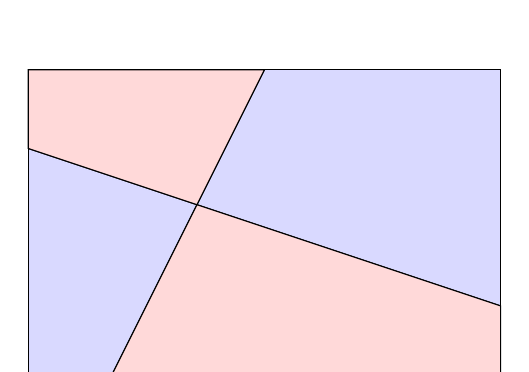
\begin{tikzpicture}
		\coordinate (A) at (0,0);
		\coordinate (B) at (2,4);
		\coordinate (C) at (-1,3);
		\coordinate (D) at (5,1);
		\filldraw[fill=blue!15!white, draw=black] (-1,0) rectangle (5,4);
		%\filldraw[fill=red, draw=black] (0,0) -- (5,0) -- (5,4) -- cycle;
		\draw (A) -- (B);
		\draw (C) -- (D);
		\coordinate (E) at (intersection of  A--B and C--D);
		\filldraw[fill=red!15!white, draw=black] (A) -- (E) -- (D) -- (5,0) -- cycle;
		\filldraw[fill=red!15!white, draw=black] (C) -- (E) -- (B) -- (-1,4) -- cycle;
	\end{tikzpicture}
\end{center}
\captionof{figure}{Example of a two-colourable map.}
\begin{theorem}[Two Colour Theorem]
	Let $P(n)$ denote the statement "Any map of the above form with n lines is two-colourable". Then, it holds that $\forall n \in\mathbb{N}$, $P(n)$.
\end{theorem}
\begin{proof}
	We shall proceed by induction.
	
	\textbf{\underline{Base Case}}: First, let us begin with the base case where $n=0$. In this case, since we have $n=0$ lines, then the map can be coloured using a single colour. Thus, $P(0)$ holds true.
	
	\textbf{\underline{Induction Hypothesis}}: Next, we shall introduce our induction hypothesis: suppose that for $n=k\geq0$, assume that $P(k)$ is true.
	
	\textbf{\underline{Inductive Step}}: Now, we begin our inductive step: we want to prove that for a map with $k+1$ lines, the map is two-colourable.
	
	Given a map with $k+1$ lines, let us first remove a line. Now, we have a map with $k$ lines and, by our induction hypothesis, it is two-colourable. 
	
	Now, observe that for a valid map colouring, swapping the colours will result in a still-valid colouring. With this observation in mind, let us add back the line we removed earlier. Now, on one side, we keep the colours the same; however, on the other side, we shall swap the colours. We claim that this is a valid two-colouring of the map with k+1 lines. Thus, we claim that $\forall n \in \mathbb{N}$, $P(n)$.
\end{proof}

\subsection{Strengthening the Induction Hypothesis} When using induction, it's important to choose the correct statement to prove. We will see this importance in the following example:

Suppose we want to prove that, for all $n\geq 1$, the sum of the first $n$ odd numbers is a perfect square.

Let's attempt to prove this with induction:
\begin{proof}[Proof attempt]\renewcommand{\qedsymbol}{$\boxtimes$}
	We shall proceed by induction on $n$.
	
	\textbf{\underline{Base Case}}: First, let us prove for the base case of $n=1$. We see that the first odd number is $1$, which is a perfect square.
	
	\textbf{\underline{Induction Hypothesis}}: Next, let us proceed with our induction hypothesis. Suppose that the sum of the first $k\geq1$ odd numbers is a perfect square, $m^2$.
	
	\textbf{\underline{Inductive Step}}: Now, our inductive step. We want to prove that our induction hypothesis holds for the first $k+1$ odd numbers. The $(k+1)^{th}$ odd number is $2k+1$. Then, by our induction hypothesis, we see that the sum of the first $k+1$ odd numbers is equal to $m^2+2k+1$.
\end{proof}

However, we see that we are now stuck; why is it that $m^2+2k+1$ has to be a perfect square?

Our induction hypothesis is too "weak" and doesn't give enough structure for us to say anything meaningful about the $(k+1)$ case. So, what do we do?

Well, first, let's take a step back to make sure that our claim isn't wrong. To do this, let's check the first few cases:

\begin{itemize}
	\item $n=1$: $1=1=1^2$
	\item $n=2$: $1+3=4=2^2$
	\item $n=3$: $1+3+5=9=3^2$
	\item $n=4$: $1+3+5+7=16=4^2$
\end{itemize}

Notice here that our claim isn't wrong. However, what is interesting is that the sum of the first $n$ odd numbers isn't just a perfect square; it is actually $n^2$. With this in mind, let us instead use a stronger claim.

\begin{theorem}
	For all $n\geq1$, the sum of the first $n$ odd numbers is equal to $n^2$.
\end{theorem}
\begin{proof}
	We shall proceed by induction on $n$,
	
	\textbf{\underline{Base Case}}: Let us first begin with the base case $n=1$. The first odd number is $1$, which is equal to $1^2$.
	
	\textbf{\underline{Induction Hypothesis}}: Next, we shall introduce our induction hypothesis: assume that the sum of the first $n=k\geq1$ odd numbers is equal to $k^2$.
	
	\textbf{\underline{Inductive Step}}: Now, our inductive step: we want to prove that our induction hypothesis holds for the first $(k+1)$ odd numbers. Notice that the $(k+1)^{th}$ odd number is $2k+1$. Then, the sum of the first $(k+1)$ odd numbers is equal to $k^2+(2k+1)=(k+1)^2$. Thus, by the principle of induction, the theorem holds.
\end{proof}

Let's look at a second example:

Suppose that we want to prove that for $n\geq 1$, $\sum{i=1}{n}\frac{1}{i^2}\leq2$.

Once again, let's try using induction:

\begin{proof}[Proof attempt]\renewcommand{\qedsymbol}{$\boxtimes$}
	We shall proceed by induction on $n$.
	
	\textbf{\underline{Base Case}}: First, we look at our base case $n=1$: we see that $\frac{1}{1^2}=1\leq2$.
	
	\textbf{\underline{Induction Hypothesis}}: Next, our induction hypothesis: let us assume that for $n=k\geq1$, $\sum{i=1}{k}\frac{1}{i^2}\leq2$.
	
	\textbf{\underline{Inductive Step}}: Now, for our inductive step, we want to prove that our induction hypothesis holds for the $(k+1)$ case:
	
	\begin{align*}
		\sum{i=1}{k+1}\frac{1}{i^2}=\sum{i=1}{k}\frac{1}{i^2}+\frac{1}{k+1} \leq 2
	\end{align*}
	
\end{proof}

But, how do we show that the last line is true? What if $\sum{i=1}{k}\frac{1}{i^2}$ is actually equal to $2$...?

Instead, let us try and strengthen our induction hypothesis.

\begin{theorem}
	For all $n\geq1, \sum{i=1}{n}\frac{1}{i^2}\leq2-\frac{1}{n}$.
\end{theorem}
\begin{proof}
	We shall proceed by induction on $n$.
	
	\textbf{\underline{Base Case}}: For the base case of $n=1$, we see that $\sum{i=1}{i}\frac{1}{i^2}=1\leq2-\frac{1}{1}$. Thus, our base case holds.
	
	\textbf{\underline{Induction Hypothesis}}: Next, we shall introduce our induction hypothesis: assume that for all $n=k\geq1$, $\sum{i=1}{k}\frac{1}{i^2}\leq2-\frac{1}{k}$.
	
	\textbf{\underline{Inductive Step}}: Now, our inductive step: we want to prove that our induction hypothesis holds for $n=k+1$:
	
	\begin{align*}
		\sum{i=1}{k+1}\frac{1}{i^2}=\sum{i=1}{k}\frac{1}{i^2}+\frac{1}{k+1} &\leq 2 - \frac{1}{k} + \frac{1}{(k+1)^2} \\
		-\frac{1}{k}+\frac{1}{(k+1)^2} &\leq -\frac{1}{k+1} \\
		-\frac{k+1}{k}+\frac{1}{k+1}&\leq-1 \\
		-(k+1)^2 + k &\leq -(k+1)(k) \\
		-(k^2+2k+1)+k &\leq -(k^2+k) \\
		k^2 + 3k + 1 &\geq k^2+k \\
		2k + 1 &\geq 1 \\
		k &\geq 0
	\end{align*}
	
	Now, we see that this is true as $k\geq1$. Thus, our induction hypothesis holds for the $(k+1)$ case. Therefore, by the principle of induction, our claim holds.
\end{proof}

\subsection{Strong Induction} So far, we've looked at what's referred to as $\textit{weak}$ induction. In this subsection, we'll look at what's known as $\textit{strong}$ induction.

So, what is strong induction exactly? Well, it's similar to simple induction. However, instead of just assuming that $P(k)$ is true, we assume that $P(0)$, $P(1),\ldots,$ $P(k)$ is true. In other words, we assume that $\land_{i=0}^k P(i)$ is true.

There isn't a difference between the power of either inductions; in other words, there aren't scenarios where one type of induction can prove a statement but the other can't. But, choosing the correct type of induction can make proofs become easier.

Now, let us look at an example of using strong induction:
\begin{theorem}
	For every natural number $n \geq 12$, it holds that $n = 4x+5y$ for some $x,y \in \mathbb{N}$.
\end{theorem}
\begin{proof}
	We proceed by induction on $n$.
	
	\underline{\textbf{Base Case}}: First, we look at the base case of $n=12$. We see that $12=4(3)+5(0)$. Thus, our claim holds for $n=12$.
	
	Next, we look at $n=13$. We observe that $13=4(2)+5(1)$. Thus, we see that $n=13$ can be expressed as $4x+5y$ for some $x,y\in \NN$.
	
	Now, we look at $n=14$, observing that $14=4(1)+5(2)$. Thus, our claim holds for $n=14$.
	
	Finally, we observe that when $n=15$, $15=4(0)+5(3)$. Therefore, our claim holds for the base case $n=15$.
	
	\underline{\textbf{Induction Hypothesis}}: Suppose that for $12 \leq n \leq k$, and for $k \leq 15$, $k=4x+5y$ for some $x,y \in \NN$.
	
	\underline{\textbf{Inductive Step}}: Now, we want to show that our induction hypothesis holds for $n=k+1 \geq 16$. Now, notice here that $(k+1)-4 \geq 12$, and from here we see that our induction hypothesis implies that for some $x', y' \in \NN$, $(k+1)-4 = 4x'+5y'$. Therefore, $(k+1)-4 = 4x + 5y$ for $x=x'+1$ and $y=y'+1$.
	
	Thus, we see that our claim holds for every natural number $n \geq 12$ by the principle of mathematical induction.
\end{proof}
	Next, we will look at a tougher example which involves strong induction:
	\begin{thm}
		Every natural number $n > 1$ can be written as a product of one or more primes.
	\end{thm}
	\begin{proof}
		We shall proceed by induction on $n$.
		
		\underline{\textbf{Base Case}}: First, we look at the base case of $n=2$. We see that since $2$ is a prime number, then our claim holds.
		
		\underline{\textbf{Induction Hypothesis}}: Suppose that our claim holds true for all $2 \leq n \leq k$.
		
		\underline{\textbf{Inductive Step}}: Now, we want to show that our induction hypothesis holds for $n=k+1$. At this point, we have two cases:
		\begin{enumerate}
			\item $k+1$ is a prime number
			\item $k+1$ isn't a prime number.
		\end{enumerate}
	
		In the first case, we see that since $k+1$ is a prime number, then our induction hypothesis holds.
		
		For the second case, if $k+1$ isn't a prime number then, by definition, $k+1 = xy$ for some $x, y \in \ZZ^{+}$, where $1 < x,y < k+1$. Now, by the induction hypothesis, we see that both $x$ and $y$ can each be written as a product of one or more primes. Then, this means that $xy=k+1$ can also be written as a product as one or more primes.
		
		Therefore, by mathematical induction, we conclude that our claim holds for every natural number $n > 1$.
	\end{proof}
\subsection{The Well-Ordering Principle}

We will now introduce a concept which is equivalent to induction: the Well-Ordering Principle.
\begin{defn}[Well-Ordering Principle]
	If $S \subseteq \NN$, and $S \not= \emptyset$, then $S$ must have a smallest element. 
\end{defn}

We observe that while using induction, our statement of ``for all $k$, $P(k) \implies P(k+1)$" only makes sense if there is a well-defined order imposed upon the natural numbers (that is, $3$ comes before $4$, $4$ before $5$, etc.). This particular property will be used later as an alternate proof to a lemma.

Now, while $\NN$ follows the Well-Ordering Principle, not all sets do.
\begin{example}
	Consider the following sets, and whether they follow the well-ordering principle or not:
	\begin{itemize}
		\item $S_{1} = \left\{  n \in \NN : n \text{ is prime}\right\}$; yes, the smallest element is $2$.
		\item $S_{2} = \left\{  n \in \ZZ\right\}$; no, there is no lower bound.
		\item $S_{3} = \left\{  n \in \ZZ^{+} \right\}$; yes, the smallest element is $1$.
	\end{itemize}
\end{example}

\begin{rmk}
	What is interesting to note is that the Well-Ordering Principle is actually not a theorem, but rather an axiom; it is part of the definition of $\NN$.
\end{rmk}

\section{Recursion, Programming, and Induction}

If it isn't clear already, there's a very strong connection between the idea of recursion in programming and induction.  We will be demonstrating this with the following two examples:
\begin{example}[Fibonacci's Rabbits]
	Consider the following puzzle: starting with a pair of rabbits, how many rabbits are there after a year, if each month each pair begets a new pair which, from the second month on, becomes productive?
	
	This model of population growth can be modeled by recursively defining a function $F(n)$; the resulting sequence is now referred to as the \textit{Fibonacci numbers}.

	Using induction, we can also show that there is a lower bound to the exponential growth of Fibonacci numbers, which will be shown in Problem 2.1.

	Now, as a program, it looks as such:
	\begin{lstlisting}[language=Python]
	def fib(n):
		if n==0 or n==1:
			return n
		else:
			return fib(n-1) + fib(n-2)
	\end{lstlisting}
	Now, we can use induction to show that, in order to find $F(n)$, the number of calls to $F(n)$ is at least $F(n)$ itself. This will be demonstrated later as an exercise problem.
\end{example}
\begin{example}[Binary Search]
	For this example, we will be using induction to analyse a recursive algorithm: the binary search.
	
	The code is as follow, in pseudocode:
	\begin{lstlisting}
	findWord(W, D) {
	if (D has precisely one page)
		Look for W in D by brute force.
		If found, return its definition; else, return "W not found".
	Let W' be the first word on the middle page of D.
	if (W comes before W')
		return findWord(first half of D)
	else
		return findWord(second half of D)
	}
	\end{lstlisting}

	Now, we will use induction to show that our function is correct.
	\begin{proof}
		We shall proceed by induction on $n$, the number of pages in $D$.
		
		\underline{\textbf{Base Case}}: If $n=1$, we observe that the function will find $W$ in $D$ by brute force, returning either the definition or that the word isn't found as desired.
		
		\underline{\textbf{Induction Hypothesis}}: Assume that the function is correct for all $1 \leq n \leq k$.
		
		\underline{\textbf{Inductive Step}}: We will show that the function works for $n=k+1$ as well. Notice that we know the word $W$ must be in either the first or second half of $D$ depending its position compared to $W'$. In either cases, we will then recurse through at most $k$ pages and thus, by our induction hypothesis, it will either return the definition or that the word isn't found.
		
		Therefore, by the principle of mathematical induction, our function is correct.
	\end{proof}
\end{example}

From these examples, it should be clear how intimate the ideas of recursion and induction are to one another.

\section{Exercises}
\begin{hw}
	Use induction to show that $F(n) \geq 2^{(n-1)/2}$ for all $n \geq 3$.
\end{hw}
\begin{proof}
	We shall proceed by induction on $n$.
	
	\underline{\textbf{Base Case}}: First, we see that for $n=3$, $F(3) = 2 \geq 2^{(3-1)/2}$. 
	
	Next, for $n=4$, we observe that $F(4)=F(3)+F(2)=3 \geq 2^{(4-1)/2} = 2.828$.
	
	Therefore, our claim holds for the base cases of $n=3$ and $n=4$.
	
	\underline{\textbf{Induction Hypothesis}}: For all $3 \leq n \leq k$, $F(k)\geq 2^{(k-1)/2}$. 
	
	\underline{\textbf{Inductive Step}}: Now, we want to show that our claim holds for $n=k+1$. Observe that $F(k+1) = F(k) + F(k-1)$. Then, we see that by our induction hypothesis, $F(k) \geq 2^{(k-1)/2}$ and $F(k-1) \geq 2^{(k-2)/2}$. Then, we observe the following:
	\begin{align*}
		F(k) + F(k-1) &\geq 2^{(k-1)/2} + 2^{(k-2)/2} \\
		&= 2^{k/2}(2^{-1/2} + 2^{-1}) \\
		&> 2^{k/2} \tag{because $2^{-1/2}+2 > 1$}
	\end{align*}
	
	Thus, we see that our claim holds true for $n=k+1$.
	
	Therefore, by mathematical induction, we can conclude that our claim holds for all $n \geq 3$.
\end{proof}
\begin{hw}
	Using induction, show that to compute $F(n)$ using our function \lstinline[language=Python]|fib(n)|, we need at least $F(n)$ calls.
\end{hw}
\begin{proof}
	We shall proceed by induction on $n$.
	
	\underline{\textbf{Base Case}}: First, we see that for $n=0$, $F(0)=0$, and it requires one call.
	
	For $n=1$, $F(1)=1$, and also requires one call to compute the value.
	
	For $n=2$, we see that $F(2)=F(1)+F(0)=1$ requires two calls to \lstinline[language=Python]|fib(n)|.
	
	For $n=3$, we observe that $F(3)=F(2)+F(1)=2$, which requires three calls to the function.
	
	For $n=4$, we see that $F(4)=F(3)+F(2)=3$, which requires 5 calls to the function to compute the result.
	
	Thus, we see that our claim holds for these base cases.
	
	\underline{\textbf{Induction Hypothesis}}: Now, for all $0 \leq n \leq k$, assume that our claim holds.
	
	\underline{\textbf{Inductive Step}}: We want to now prove that for $n=k+1$, we require at least $F(k+1)$ calls to compute $F(k+1)$. Now, we see that on the first call to \lstinline[language=Python]|fib| with $k+1$, the function will then call on \lstinline[language=Python]|fib(k)| and \lstinline[language==Python]|fib(k-1)|. Then, by our inductive hypothesis, each of these calls will take at least $F(k)$ and $F(k-1)$ calls respectively to calculate the results. Then, we see that we need at least $F(k)+F(k-1)$ calls to compute $F(k+1)$ which, by definition, is $F(k+1)$ calls. Thus, our claim holds for $n=k+1$.
	
	Therefore, by the mathematical principle of induction, our claim holds true for all $n \geq 0$, where $n \in \NN$.
\end{proof}
\begin{hw}
	Prove that for any natural number $n \geq 1$, $\sum{i=1}{n} i^{2}=\dfrac{1}{6}n(n+1)(2n+1)$.
\end{hw}
\begin{proof}
	We shall proceed by induction on $n$.
	
	\textbf{\underline{Base Case}}: First, consider our base case $n=1$. We see that $1^{2}=\dfrac{1}{6}(1)(1+1)(2(1)+1)=1$. Thus, our claim holds for the base case of $n=1$.
	
	\underline{\textbf{Induction Hypothesis}}: Now, suppose that for $n=k$, where $k \geq 1$, our claim holds true.
	
	\underline{\textbf{Inductive Step}}: We want to show that our induction hypothesis holds for $n=k+1$. Observe the following:
	\begin{equation*}
		\sum{i=1}{k+1} i^{2} = \sum{i=1}{k} i^{2} + (k+1)^{2}
	\end{equation*}

	Now, by our induction hypothesis, we see the following:
	\begin{align*}
		\sum{i=1}{k} i^{2} + (k+1)^{2} &= \dfrac{k(k+1)(2k+1)}{6} + (k+1)^{2} \\
		&= \dfrac{k(k+1)(2k+1)+6(k+1)^{2}}{6} \\
		&= \dfrac{(k+1)(k)(2k+1)+6(k+1)^{2}}{6} \\
		&= \dfrac{(k+1)(2k^{2}+k+6(k+1))}{6} \\
		&= \dfrac{(k+1)(2k^{2}+7k+6)}{6} \\
		&= \dfrac{(k+1)(k+2)(2k+3)}{6} \\
		&= \dfrac{(k+1)((k+1)+1)(2(k+1)+1)}{6}
	\end{align*}

	Therefore, our induction hypothesis holds for $n=k+1$. Thus, by mathematical induction, we can conclude that our claim holds true for all natural number $n \geq 1$.
\end{proof}
\begin{hw}[Bernoulli's Inequality]
	Prove that $(1+x)^{n} \geq 1+nx$ if $n$ is a natural number and $1+x > 0$.
\end{hw}
\begin{proof}
	We shall proceed by induction on $n$.
	
	\underline{\textbf{Base Case}}: First, we see that for $n=0$, then $(1+x)^{0} = 1 = 1+(0)x$. Therefore, the claim holds for our base case of $n=0$.
	
	\textbf{\underline{Induction Hypothesis}}: Next, suppose that for $n=k$, where $k \geq 0$, $(1+x)^{k} \geq 1+kx$ if $k \in \NN$ and $1+x > 0$.
	
	\textbf{\underline{Inductive Step}}: Now, we want to show that our claim holds for $n=k+1$. Observe that for $k+1$, $(1+x)^{k+1}=(1+x)^{k}(1+x)$. Then, we observe the following:
	\begin{align*}
		(1+x)^{k+1} &= (1+x)^{k}(1+x) \\
		&\geq (1+kx)(1+x) \tag{by our induction hypothesis} \\
		&= 1+kx+x+kx^{2} \\
		&\geq 1 + kx + x \tag{as $k, x^{2} \geq 0$} \\
		&= (1+(k+1)x)
	\end{align*}

	Thus, we see that for $n=k+1$, $(1+x)^{k+1} \geq 1+(k+1)x$.
	
	Therefore, by the principle of mathematical induction, we can conclude that our claim holds for all $n \in \NN$.
\end{proof}
\begin{hw}
	A common recursively defined function is the \textit{factorial}, defined for a nonnegative number $n$ as $n! = n(n-1)(n-2) \ldots 1$, with base case $0! = 1$. Let us reinforce our understanding of the connection between recursion and induction by proving the following:
	\begin{equation*}
		\forall n \in \NN\text{, }n > 1 \implies n! < n^{n}
	\end{equation*}
\end{hw}
\begin{proof}
	We shall proceed by induction on $n$.
	
	\textbf{\underline{Base Case}}: We first consider the base case of $n=2$. For $n=2$, we see that $2!=2$, and $2^{2}=4$. Therefore, $n! < n^{n}$ for $n=2$, and our base case holds.
	
	\textbf{\underline{Induction Hypothesis}}: Assume that our claim holds true for $n=k$, where $k \geq 2$.
	
	\textbf{\underline{Inductive Step}}: Now, we want to show that our claim holds true for $n=k+1$. Notice that $(k+1)! = (k+1)k!$. Now, by our induction hypothesis, we know that $(k+1)k! < (k+1)k^{k}$. From here, observe the following:
	\begin{align*}
		(k+1)^{k+1} &= (k+1)^{k}(k+1) \\
		k^{k}(k+1) &< (k+1)^{k}(k+1) \\
		(k+1)k! &< k^{k}(k+1) \\
		&< (k+1)^{k}(k+1) \\
		\therefore (k+1)k! &< (k+1)^{k+1}
	\end{align*}

	Since our claim holds for $n=k+1$ as well then, by the principle of mathematical induction, our claim holds for all $n > 1$.
\end{proof}

\newpage

\chapter{Stable Matching}
\section{The Stable Matching Problem}
In the previous two chapters, we examined proof techniques; now, we will look at how we can apply them to an important problem referred to as the \textit{Stable Matching Problem}.

The Stable Matching problem is as follows:

\begin{defn}[The Stable Matching Problem]
	Suppose we have an employment system, and we have to match up $n$ jobs and $n$ candidates. In this case, $n=3$. Below are a list of jobs and candidates, along with a preference list:

	\begin{center}
		\begin{tabular}{|c|c|}
		\hline
		Jobs & Candidates \\
		\hline
		$A$ & $X > Y >Z$ \\
		\hline
		$B$ & $Y > X > Z$ \\
		\hline
		$C$ & $X > Y > Z$ \\
		\hline
		\end{tabular}
	
		\bigskip
		
		\begin{tabular}{|c|c|}
			\hline
			Candidates & Jobs \\
			\hline
			$X$ & $B > A > C$ \\
			\hline
			$Y$ & $A > B > C$ \\
			\hline
			$Z$ & $A > B > C$ \\
			\hline
		\end{tabular}
	\end{center}
	\captionof{table}{The preference lists of the jobs and candidates.}
	
	Now, how would we match each job to each candidate such that everybody is ``happy"? Not any type of matching would suffice. Can we do it efficiently?
\end{defn}

Now, it turns out that there exists an algorithm that helps achieve this: the \textit{Propose-and-Reject Algorithm} (referred to as the Gale-Shapley Algorithm), which we will present now.
\newpage

\section{The Propose-and-Reject Algorithm}
\begin{defn}[Propose-and-Reject Algorithm]
	We think of the algorithm as proceeding in ``days" to have a clear unambiguous sense of discrete time.
	
	\textbf{Every Morning}: Each job proposes (i.e. makes an offer) to the most preferred candidate on its list who has not yet rejected this job.
	
	\textbf{Every Afternoon:} Each candidate collects all the offers she received in the morning; to the job offer she likes best among these, she responds ``maybe" (she now has it \textit{on a string}), and rejects the other offers. 
	
	\textbf{Every Evening}: Each rejected job crosses off the candidate who rejected its offer from its list.
	
	The above loop is repeated each successive day until there are no offers rejected. At that point, each candidate has a job offer on a string; and on this day, each candidate accepts their offered job and the algorithm terminates.
\end{defn}

Now, to understand this algorithm later, let's look at the example given earlier and see it in action:
\begin{example}
	The following table will show how the algorithm plays out, showing which jobs makes an offer to which candidate on the given day:
	
	\begin{center}
		\begin{tabular}{|c|c|c|}
			\hline
			Days & Candidates & Offers \\
			\hline
			\multirow{3}{2em}{\centering $1$} & $X$ & $A > C$ \\
			& $Y$ & $B$ \\
			& $Z$ & --- \\
			\hline
			\multirow{3}{2em}{\centering $2$} & $X$ & $A$ \\
			& $Y$ & $B > C$ \\
			& $Z$ & --- \\
			\hline
			\multirow{3}{2em}{\centering $3$} & $X$ & $A$ \\
			& $Y$ & $B$ \\
			& $Z$ & $C$ \\
			\hline
		\end{tabular}
	\end{center}
\captionof{table}{Depiction of the Propose-and-Reject algorithm.}

	And thus, the algorithm ends after three days with the following pairings: $\left\{  (X, A), (Y, B), (Z, C)\right\}$
\end{example}

\subsection{Properties of the Propose-and-Reject Algorithm}

There are two properties which we shall show about the algorithm:
\begin{enumerate}
	\item The Propose-and-Reject algorithm halts.
	\item The algorithm outputs a ``good" (i.e. stable) matching.
\end{enumerate}

Now, looking at these two properties, we notice that in order to prove the second property, we must first define what a ``stable" matching actually entails.

\subsubsection{Stability}
\begin{defn}[Rogue Couple]
	A rogue couple is where a job $J$ and a candidate $C$ both prefer working with each other over their current matching. This is demonstrated in the following diagram:
	
	\begin{center}
		\tikz{
		\begin{scope}[name prefix = top-]
			\node (J) at (0,1) {$J$};
			\node (C) at (1,1) {$C$};
			\draw (J) -- (C);
		\end{scope}
		\begin{scope}[name prefix = bottom-]
			\node (J') at (0,0) {$J'$};
			\node (C') at (1,0) {$C'$};
			\draw (J') -- (C');
		\end{scope}
		\draw[dashed][red][stealth-stealth] (top-C) -- (bottom-J');
		}
	\end{center}
	\captionof{figure}{Visualisation of a rogue couple.}

	In the example above, we see that the rogue couple would be the pair (J', C), as they \textit{both} prefer each other. The diagram above is what's referred to as an unstable matching.
\end{defn}

So, what exactly is a ``stable matching"? Well, it's a matching where there aren't any rogue couples.

What is important to note here is that for it to be a rogue couple, both the job and the candidate have to prefer each other! If C prefers J' but J' prefers C' over C, then it is still a stable matching!

For example, let's go back to our previous example:
\begin{example}
	Recall our previous example:
	
	\begin{center}
		\begin{tabular}{|c|c|}
			\hline
			Jobs & Candidates \\
			\hline
			$A$ & $X > Y >Z$ \\
			\hline
			$B$ & $Y > X > Z$ \\
			\hline
			$C$ & $X > Y > Z$ \\
			\hline
		\end{tabular}
		
		\bigskip
		
		\begin{tabular}{|c|c|}
			\hline
			Candidates & Jobs \\
			\hline
			$X$ & $B > A > C$ \\
			\hline
			$Y$ & $A > B > C$ \\
			\hline
			$Z$ & $A > B > C$ \\
			\hline
		\end{tabular}
	\end{center}

	We found that a stable matching is $\left\{  (X, A), (Y, B), (Z, C)\right\}$. However, we notice that $X$ prefers job $B$, so how is this a stable matching? 
	
	Well, while $X$ prefers $B$, $B$ doesn't prefer $X$ over $Y$. Similarly, although $Y$ would prefer job $A$ over $B$, job $A$ prefers $X$ over $Y$. Also, notice here that job $C$ and candidate $Z$ are stuck with each other; it is possible in a stable matching to be stuck with your least preferred option.
	
	Below is a diagram of the scenario which helps to clarify the situation:
	
	\begin{center}
		\tikz{
			\begin{scope}[name prefix = top-]
				\node (A) at (0,2) {$A$};
				\node (X) at (1,2) {$X$};
				\draw (A) -- (X);
			\end{scope}
			\begin{scope}[name prefix = mid-]
				\node (B) at (0,1) {$B$};
				\node (Y) at (1,1) {$Y$};
				\draw (B) -- (Y);
			\end{scope}
			\begin{scope}[name prefix = bot-]
				\node (C) at (0,0) {$C$};
				\node (Z) at (1,0) {$Z$};
				\draw (C) -- (Z);
			\end{scope}
			\draw[dashed][red][-stealth] (top-X) -- (mid-B);
			\draw[dashed][red][-stealth] (mid-Y) -- (top-A);
		}
	\end{center}
	\captionof{figure}{A figure explaining stable matching.}
\end{example}

Now, before we discuss how to find a stable matching, we first have to ask a more basic question: do stable matchings always exist?

At first, it may seem as though the answer is yes: if a rogue couple exists, we can simply pair them up, right? However, while this does reduce the number of rogue couples by one, it might then also create a new rogue couple. So, it isn't clear whether the algorithm ends or not.

\begin{example}[Roommates Problem]
	We will illustrate the fallacy of the reasoning above through this example.
	
	We have $2n$ people who must be paired up to be roommates. The difference between this problem and the Propose-and-Reject algorithm is that the latter has asymmetric partners of a different type, where here a person can be paired up with any of the other $2n-1$ people --- there is no asymmetry in type.
	
	Now, using the line of reasoning prior, if there was a rogue couple, we could simply just match them up iteratively until there are no rogue couples. Since this approach doesn't take advantage of the asymmetry, it can be applied to the scenario.
	
	However, this doesn't work. Let's look at the following counterexample:
	
	\begin{center}
		\begin{tabular}{|c|ccc|}
			\hline
			\multicolumn{4}{|c|}{Roommates} \\
			\hline
			$A$ & $B$ & $C$ & $D$ \\
			\hline
			$B$ & $C$ & $A$ & $D$ \\
			\hline
			$C$ & $A$ & $B$ & $D$ \\
			\hline
			$D$ & --- & --- & --- \\
			\hline
		\end{tabular}
	\end{center}
\captionof{table}{Illustration of the Roommates Problem.}

	We claim that in this example, there's a rogue couple for any matching:
	\begin{itemize}
		\item 	$\left\{  (A,B), (C,D) \right\}$ would result in a rogue matching, with rogue couple $(B, C)$. 
		\item $\left\{ (B,C), (A,D) \right\}$ would result in a rogue matching, with rogue couple $(A,C)$. 
		\item $\left\{  (A,C), (B,D) \right\}$ would result in a rogue matching, with rogue couple $(A,B)$.
	\end{itemize}

	And thus, we see that there can never be a stable matching.
\end{example}

From this example, we see that any proof showing that there always exists a stable matching must exploit the asymmetry in types.

\subsection{Proofs of Properties}
We will now prove the first property of the algorithm:
\begin{lem}
	The propose-and-reject algorithm always halts.
\end{lem}
\begin{proof}
	We shall proceed by direct proof.
	
	Observe that for every day that the algorithm doesn't stop, at least one job has to eliminate some candidate from its list (if not then the algorithm's halting condition would activate). Therefore, as there are $n$ elements in $n$ lists, that means that it takes at most $n^{2}$ days for the algorithm to terminate.
\end{proof}

Next, we will prove the second property. First, let us make an observation:
\begin{obs}
	Each job begins the algorithm with its first choice as a possibility. However, as time progresses, its best available option gets worse. Meanwhile, the candidate's offers can only get better over time.
\end{obs}
From this, we see intuitively that at some point the jobs and candidates must ``meet" in the middle, which is where a stable match occurs.

Now, let us formalise this and prove it as well:
\begin{lem}[Improvement Lemma]
	If job $J$ makes an offer to a candidate $C$ on the $k^{th}$ day, then on every subsequent day $C$ has an offer on a string which they like as much as job $J$.
\end{lem}
\begin{proof}
	We shall proceed by induction on $n$.
	
	\textbf{\underline{Base Case}}: First, we consider the case of $k=i$. On the $i^{th}$ day, if $C$ receives at least one offer, one of which is by $J$, then at the end of the day they will have either an offer from $J$ or from a job $J'$ which they like more.
	
	\textbf{\underline{Induction Hypothesis}}: We suppose that for some $i \geq k$, our claim holds true.
	
	\textbf{\underline{Inductive Step}}: We will now prove our claim for $k=i+1$. We observe that, by the induction hypothesis, on day $i$, $C$ would have had an offer from a job $J'$ which they like at least as much as the offer from job $J$. Now, on the $(i+1)^{th}$ day, $J'$ gives $C$ an offer again; at the end of the day, $C$ will have either $J'$ on a string, or another offer from a job which they like more than $J'$.
	
	In both cases, we observe that the job $C$ has on a string is one they like at least as much $J$. Therefore, we see that our claim holds for $k=i+1$.
	
	Thus, by the principle of mathematical induction, our claim holds for all $k \in \NN$.
\end{proof}

Now, we will show an alternate proof for the Improvement Lemma, using the Well-Ordering Principle:
\begin{proof}[Proof (using Well-Ordering Principle)]
	As with the original proof, we observe that the claim holds for day $k=i$. Now, suppose, for contradiction, that the $i^{th}$ day, where $i > k$, is the first counterexample where $C$ has either no offer on a string or an offer from a job $J^{*}$ they like less than $J$.
	
	Now, on day $i=1$, $C$ had an offer from some job $J'$ which they liked at least as much as $J$. According to the algorithm, on day $i$, $J'$ will make an offer to $C$ again; then, $C$ has the choice of at least one job $J'$. As such, $C$'s best choice has to be at least as good as $J'$, and it would definitely be better than having no offer or an offer from $J^{*}$. Thus, we observe a contradiction.
	
	Therefore, we see that the Improvement Lemma holds true.
\end{proof}

We see that in the alternate proof using the Well-Ordering Principle, when we assume that there's a first counterexample on the $i^{th}$ day; this notion of a first counterexample wouldn't be valid if $\NN$ didn't have a well-defined order.

\chapter{Graph Theory}
\section{Introduction}
One of the core ideas of computer science is abstraction; that is, representing a complex situation with a simple model. Examples includes the brain, the Internet, maps, etc.

And in all of these cases, there is an underlying ``network" --- ``graphs" --- that helps us understand these entities more deeply.

The origin of graph theory stems back to K\"{o}nigsberg, Prussia. Through their city ran the Pregel river, the city into two banks $A$ and $C$ and islands $B$ and $D$. Connecting the islands to the mainland were seven bridges. The residents tried to figure out a path which would allow them to cross each of the seven bridges exactly once. Below is a representation of this problem using a graph:

\begin{center}
	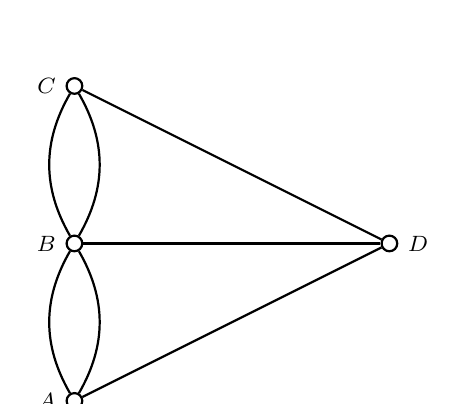
\begin{tikzpicture}
		[lineDecorate/.style={-,thick},%                                                
		nodeDecorate/.style={shape=circle,inner sep=2pt,draw,thick}]
		%% nodes or vertices                                                            
		\foreach \nodename/\x/\y/\direction/\navigate in {
			A/0/0/left/west, B/0/2/left/west, C/0/4/left/west, D/4/2/right/east}
		{
			\node (\nodename) at (\x,\y) [nodeDecorate] {};
			\node [\direction] at (\nodename.\navigate) {\footnotesize$\nodename$};
		}
		%% edges or lines                                                               
		\path
		\foreach \startnode/\endnode in {A/D, B/D, C/D}
		{
			(\startnode) edge[lineDecorate] node {} (\endnode)
		}
		\foreach \startnode/\endnode in {A/B, B/C, C/B, B/A}
		{
			(\startnode) edge[lineDecorate,bend left] node {} (\endnode)
		};
	\end{tikzpicture}
\end{center}
\captionof{figure}[]{The (multi-)graph modeling of the bridge connections in K\"{o}nigsberg.}

Euler managed to prove that there was no solution; it was impossible. The key thing to this problem is that the problem is essentially: from a starting point, we have to trace through all the line segments without traversing through a line segment more than once.

Under these tracing rules, we see that the pen must enter each small circle as many times as it exists them; but since there are an odd number of line segments connected to each circle, we see that this is impossible to do!

\section{Formal Definitions}
\begin{defn}[Undirected Graph]
	An undirected graph is defined by a set of vertices $V$ and set of edges $E$. A graph is considered directed if each edge goes in both direction; i.e. $(u,v) \in E \iff (v,u) \in E$, then the graph is undirected.
\end{defn}
 Looking at Figure 4.1, we observe that the vertices corresponds to each of the small circles, while the edges corresponds to the line segment between each vertices.
 
\begin{rmk}
	 Note that in Figure 4.1, 
	 \begin{itemize}
	 	\item $V = \left\{  A, B, C, D\right\}$
	 	\item $E = \left\{  \left\{  A,B\right\}, \left\{  A,B \right\}, \left\{  A,D\right\}, \left\{ B,D\right\}, \left\{  B,C\right\}, \left\{  B,C\right\}, \left\{  C,D\right\} \right\}$
	 \end{itemize}
	 
	 We see that $E$ is a multiset (which is a set in which an element can appear more than once); however, generally we will be not considering such a situation where there are multiple edges between a single pair of vertices.
	 
	 So, in our definition, we require $E$ to be a set. If there are multiple edges, they'll be collapsed into one single edge. Thus, between any pair of verticies, there can only be $0$ or $1$ edge.
\end{rmk}

More generally, we can also define a directed graph. One way to think about the difference between the two is that while the edges in undirected graphs don't have direction, the ones in directed graphs do. More formally, we can define it as such:
\begin{defn}[Directed Graph]
	Let $V$ be a set denoting the vertices of a graph $G$. Then, the set of directed edges $E$ is a subset of $V \times V$; i.e. $E \subseteq V \times V$.
\end{defn}

\begin{example}
	Let $V = \left\{  1,2,3,4\right\}$, and $E = \left\{  (1,2), (1,3), (1,4)\right\}$. Below is the corresponding graphs for the directed graph $G_{1}$ and an undirected graph $G_{2}$:
	\begin{center}
		\begin{tikzpicture}
			\coordinate[] (1) at (0,0);
			\coordinate (2) at (0,3);
			\coordinate[] (3) at (2,2);
			\coordinate[] (4) at (2,0);
			\node[label={left: $1$}] at (1) {};
			\node[label={left: $2$}] at (2) {};
			\node[label={right: $3$}] at (3) {};
			\node[label={right: $4$}] at (4) {};
			\draw[-stealth] (1) -- (4);
			\draw[-stealth] (1) -- (2);
			\draw[-stealth] (1) -- (3);
			\foreach \Nombre in {1,2,3,4}
				\node[circle,inner sep=1pt,fill=black] at (\Nombre) {};  
		\end{tikzpicture}
		$\qquad\qquad$
		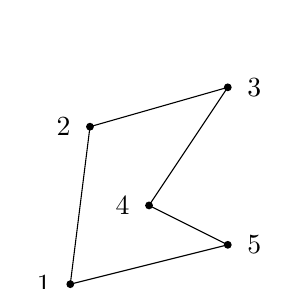
\begin{tikzpicture}
			\coordinate[] (1) at (0,0);
			\coordinate (2) at (0.25,2);
			\coordinate[] (3) at (2,2.5);
			\coordinate[] (4) at (1,1);
			\coordinate[] (5) at (2,0.5);
			\node[label={left: $1$}] at (1) {};
			\node[label={left: $2$}] at (2) {};
			\node[label={right: $3$}] at (3) {};
			\node[label={left: $4$}] at (4) {};
			\node[label={right: $5$}] at (5) {};
			\draw (1) -- (5);
			\draw (1) -- (2);
			\draw (2) -- (3);
			\draw (3) -- (4);
			\draw (4) -- (5);
			\foreach \Nombre in {1,2,3,4,5}
			\node[circle,inner sep=1pt,fill=black] at (\Nombre) {};  
		\end{tikzpicture}
	\end{center}
	\captionof{figure}[]{Examples of directed graph $G_{1}$ and undirected graph $G_{2}$, respectively.}
	
	Note that each edge in $G_{1}$ has a direction specified by an arrow; in other words, $(1,2) \in E$, but $(2,1) \not\in E$.
	
	On the other hand, in $G_{2}$, since each edge goes in both directions, we see that $(u,v) \in E$ and $(v,u) \in E$. For undirected graphs, we drop the ordered pair notation, instead denoting the edge between $u$ and $v$ by the set $\left\{  u, v\right\}$. For simplicity, we omit the arrowheads for undirected graphs.
\end{example}

From this, we conclude that a graph is formally specified as an ordered pair $G = (V,E)$, where $V$ is the vertex set and $E$ is the edge set.

Moving on from this example, we will now introduce a few more definitions.

\begin{defn}[Incident Edges]
	We say that edge $e=\left\{  u,v \right\}$ is incident on vertices $u$ and $v$.
\end{defn}
\begin{defn}[Adjacent Vertices]
	For edge $e=\left\{  u,v \right\}$, we say that vertices $u$ and $v$ are neighbours, also referred to as being adjacent.
\end{defn}
\begin{defn}[Degree]
	We have two different definitions of degree depending on whether the graph is directed or undirected:
	
	\begin{itemize}
		\item If $G$ is an undirected graph, the degree of a vertex $u \in V$ is the number of edges incident to $u$. In other words, $d(u) = \left\{  v \in V : {u,v} \in E \right\}$. A vertex $u$ with a degree of $0$ is referred to as an isolated vertex.
		
		\item If $G$ is a directed graph, there are two different types of degrees a vertex can have; the in-degree is the number of edges from other vertices to $u$, and the out-degree which is the number of edges from $u$ to other vertices.
	\end{itemize}
\end{defn}
\begin{rmk}
	Notice here that our definition of a graph allows for a self-loop; that is, we can have edges in the form of $\left\{  u,u \right\}$ or $(u,u)$. However, as this doesn't give us any useful information, in general we shall assume that graphs don't have any self-loops (unless stated otherwise).
\end{rmk}
\subsection{Paths, Walks, and Cycles}
In order to understand proofs discussing graphs, we must understand all the terms which they use.

Now, we will define a couple more things that will be essential to our understanding of graph theory, and they are especially crucial to understanding a lot of later theorems that will be discussed.
\begin{defn}[Path]
	Let $G=(V,E)$ be an undirected graph. Then, we define a path in $G$ as a sequence of edges $\left\{  v_{1}, v_{2} \right\}, \left\{  v_{2}, v_{3} \right\},\ldots, \left\{  v_{n-2}, v_{n-1}\right\}, \left\{  v_{n-1}, v_{n} \right\}$. In this case, we can say that there is a path between $v_{1}$ and $v_{n}$.
\end{defn}
\begin{rmk}
	In the class, we assume that a path is simple, meaning that $v_{1} \ldots v_{n}$ are distinct. Later on in our example, this notion will make more sense.
\end{rmk}
\begin{defn}[Cycle]
	A cycle is defined as a sequence of edges $\left\{  v_{1}, v_{2} \right\},\ldots, \left\{  v_{n-1}, v_{n} \right\}, \left\{  v_{n}, v_{1}\right\}$, where $v_{1}, \ldots, v_{n}$ are all distinct. A cycle is essentially a path that starts and end with the same vertex.
\end{defn}
\begin{defn}[Walk]
	A walk is a sequence of possibly repeated vertices.
\end{defn}
\begin{defn}[Tour]
	The relationship of a walk and a tour is analogous to a path and a cycle; a tour is simply a walk that starts and end with the same vertex.
\end{defn}
\begin{example}
	The following example will help visualise understand each of our definitions:
	\begin{center}
		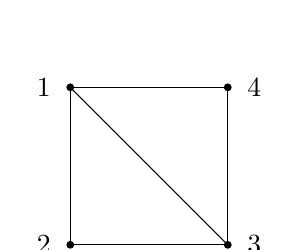
\begin{tikzpicture}
			\coordinate[] (1) at (0,2);
			\coordinate[] (2) at (0,0);
			\coordinate (3) at (2,0);
			\coordinate (4) at (2,2);
			\node [label=left:$1$] at (1) {};
			\node [label=left:$2$] at (2) {};
			\node [label=right:$3$] at (3) {};
			\node [label=right:$4$] at (4) {};
			\draw (1) -- (2) -- (3) -- (4) -- (1);
			\draw (1) -- (3);
			\foreach \Nombre in {1,2,3,4}
				\node[circle,inner sep=1pt,fill=black] at (\Nombre){};
		\end{tikzpicture}
	\end{center}
	\captionof{figure}{Undirected graph $G_{3}$, where each vertex corresponds to a house.}

	\begin{itemize}
		\item We observe that there exists multiple paths from house $1$ to house $3$ in $G_{3}$; we can either go through $2$, $4$, or directly to $3$ from house $1$.
	
		\item A possible cycle in $G_{3}$, starting from house $1$, would be the sequence: $\left\{  1, 2\right\}, \left\{  2, 3\right\}, \left\{  3, 1\right\}$.
	
		\item Now, imagine instead that we wanted to go on a leisurely stroll from house $1$ to house $3$, taking the path $\left\{  1,2\right\}, \left\{  2,1\right\}, \left\{  1, 3\right\}$. This would be a walk.
	
		\item An example of a tour would be $\left\{  1,2\right\}, \left\{  2,1\right\}, \left\{  1, 3\right\}, \left\{  3, 1\right\}$. Furthermore, note that a tour could also be a cycle. For example, the sequence of edges $\left\{  1,2\right\}, \left\{  2,3\right\}, \left\{  3,1\right\}$ would also be considered a tour.
	\end{itemize}
\end{example}
\begin{rmk}
	In the example above, we see that the notion of paths being simple makes complete sense; if we wanted to go from house $1$ to house $3$ via house $2$, there isn't a need to visit house $2$ twice.
\end{rmk}

As a short summary, below is a table detailing the differences between each of the definitions:
\begin{center}
	\begin{tabular}{cccc}
		& no repeated vertices & no repeated edges & start = end \\
		\hline
		Walk & & & \\
		\hline
		Path & \checkmark & \checkmark & \\
		\hline
		Tour & & & \checkmark \\
		\hline
		Cycle & \checkmark* & \checkmark & \checkmark \\
	\end{tabular}
\end{center}
\captionof{table}{Table explaining main differences between a walk/path/tour/cycle}
\begin{rmk}
	*Note here that we are excluding the start and end vertices.
\end{rmk}

\subsection{Connectivity}
Much of what we discuss in this chapter revolves around the idea of connectivity.
\begin{defn}[Connectivity]
	A graph is said to be connected if there is a path between any two distinct vertices. Looking at $G_{3}$ in Figure 4.3, we see that the graph is connected as we can drive from one house to another via some sequence of edges.
\end{defn}

\begin{example}
	Below, we will show examples of connected and unconnected graphs.
	
	First, recall the graphs $G_{1}$, $G_{2}$, and $G_{3}$ from previous examples. These are examples of connected graphs:
	\begin{center}
		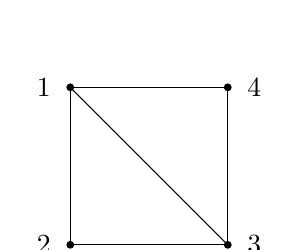
\begin{tikzpicture}
			\coordinate[] (1) at (0,2);
			\coordinate[] (2) at (0,0);
			\coordinate (3) at (2,0);
			\coordinate (4) at (2,2);
			\node [label=left:$1$] at (1) {};
			\node [label=left:$2$] at (2) {};
			\node [label=right:$3$] at (3) {};
			\node [label=right:$4$] at (4) {};
			\draw (1) -- (2) -- (3) -- (4) -- (1);
			\draw (1) -- (3);
			\foreach \Nombre in {1,2,3,4}
				\node[circle,inner sep=1pt,fill=black] at (\Nombre){};
		\end{tikzpicture}
		$\qquad\qquad$
		\begin{tikzpicture}
			\coordinate[] (1) at (0,0);
			\coordinate (2) at (0,2);
			\coordinate[] (3) at (2,2);
			\coordinate[] (4) at (2,0);
			\node[label={left: $1$}] at (1) {};
			\node[label={left: $2$}] at (2) {};
			\node[label={right: $3$}] at (3) {};
			\node[label={right: $4$}] at (4) {};
			\draw[-stealth] (1) -- (4);
			\draw[-stealth] (1) -- (2);
			\draw[-stealth] (1) -- (3);
			\foreach \Nombre in {1,2,3,4}
				\node[circle,inner sep=1pt,fill=black] at (\Nombre) {};  
		\end{tikzpicture}
		$\qquad\qquad$
		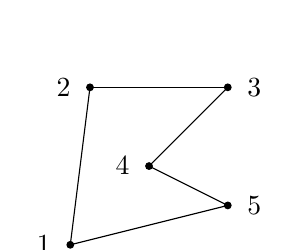
\begin{tikzpicture}
			\coordinate[] (1) at (0,0);
			\coordinate (2) at (0.25,2);
			\coordinate[] (3) at (2,2);
			\coordinate[] (4) at (1,1);
			\coordinate[] (5) at (2,0.5);
			\node[label={left: $1$}] at (1) {};
			\node[label={left: $2$}] at (2) {};
			\node[label={right: $3$}] at (3) {};
			\node[label={left: $4$}] at (4) {};
			\node[label={right: $5$}] at (5) {};
			\draw (1) -- (5);
			\draw (1) -- (2);
			\draw (2) -- (3);
			\draw (3) -- (4);
			\draw (4) -- (5);
			\foreach \Nombre in {1,2,3,4,5}
				\node[circle,inner sep=1pt,fill=black] at (\Nombre) {};  
		\end{tikzpicture}
	\end{center}
	\captionof{figure}{Examples of connected graphs.}
	
	Meanwhile, below is an example of what is considered an unconnected graph:
	\begin{center}
		\begin{tikzpicture}
			\coordinate (1) at (0,2);
			\coordinate (2) at (0,0);
			\coordinate (3) at (2,0);
			\coordinate (4) at (2,2);
			\coordinate (5) at (3,1);
			\coordinate (6) at (4,0.5);
			\coordinate (7) at (5,1.5);
			\node [label={left: $1$}] at (1) {};
			\node [label={left: $2$}] at (2) {};
			\node [label={right: $3$}] at (3) {};
			\node [label={right: $4$}] at (4) {};
			\node [label={left: $5$}] at (5) {};
			\node [label={right: $6$}] at (6) {};
			\node [label={right: $7$}] at (7) {};
			\draw (1) -- (2) -- (3);
			\draw (5) -- (7) -- (6);
			\foreach \Nombre in {1,2,3,4,5,6,7}
				\node[circle,inner sep=1pt,fill=black] at (\Nombre) {};  
		\end{tikzpicture}
	\end{center}
	\captionof{figure}{Example of an unconnected graph.}
	
	Note here that for any graph, even disconnected ones, they always consist of a collection of some connected components; i.e. sets $V_{1}, \ldots, V_{k}$ of vertices, such that all vertices in a set $V_{i}$ are connected. For example, in Figure 4.5, while the graph is unconnected, we observe that it consists of three connected components:
	\begin{itemize}
		\item $V_{1} = \left\{  1,2,3 \right\}$
		\item $V_{2} = \left\{  4 \right\}$
		\item $V_{3} = \left\{  5, 6, 7 \right\}$
	\end{itemize}
\end{example}

\section{Eulerian Tours}
Now, we shall revisit the problem that helped kickstart graph theory --- let us revisit the Seven Bridges of K\"{o}nigsberg.

Before figuring out what the problem is asking exactly, we have to first introduce two more terms:
\begin{defn}[Eulerian Walk]
	Any such walk in a graph which only visits each edge once is referred to as an ``Eulerian walk" 
\end{defn} 
\begin{defn}[Eulerian Tour]
	Moreover, if an Eulerian walk is closed, then it ends at the starting point --- this is called an Eulerian tour 
\end{defn}

Thus, going back to the problem, we see that it's asking if there exists an Eulerian tour for a given graph $G$. We now give a precise characterisation of this in terms of simpler properties of $G$. For this, we define an even degree graph as a graph where all of its vertices have an even degree.

\begin{thm}[Euler's Theorem (1736)]
	An undirected graph $G=(V,E)$ has an Eulerian tour if and only if $G$ is even degree, and connected (except possibly for isolated vertices).
\end{thm}
\begin{proof}
	In order to prove this theorem, we have to prove it for both directions. To begin with, we will prove the ``only if" direction.
	\begin{proof}[Only if]
		We shall proceed by direct proof.
		
		Let us assume that $G$ has an Eulerian tour. 
		
		We will first show that the graph is connected. As $G$ has an Eulerian tour, this means that every vertex which has an edge adjacent to it must lie on the tour, and it must be connected to every other vertices that lies on the tour. Therefore, we see that the graph is connected.
		
		Next, we will show that the graph is even degree. Notice that every time the tour enters a vertex, it has to leave the vertex via a different edge. Therefore, each vertex has two edges adjacent to it which can be paired up. 
		
		However, for the starting vertex as the edge leaving it can't be paired up, this doesn't work for the starting vertex. But, notice that by the definition of an Eulerian tour, the tour ends at the start vertex; therefore, we can pair up the first edge with the last edge entering the it. As such, we see that all the edges adjacent to a vertex can be paired up with each other, we see that each vertex has an even degree.
		
		Therefore, we can conclude that if $G$ has an Eulerian tour then $G$ is even degree and is connected.
	\end{proof}

	Next, we will prove the other direction; that is, we will prove that if a graph $G$ is even degree and is connected, then it will have an Eulerian tour.
	\begin{proof}[If]
		We shall proceed by induction on $n$, where $n$ is the number of vertices a graph $G$ has.
		
		\textbf{\underline{Base Case}}: First, for $n=2$, we observe that our graph has $2$ vertices. As the graph is even degree, it means that there must be two edges connecting the two vertices. Therefore, it has an Eulerian tour.
		
		\textbf{\underline{Induction Hypothesis}}: Now, for every graph with $2 \leq n \leq k$ vertices, we suppose that our claim holds true; that is, it will have an Eulerian tour.
		
		\textbf{\underline{Inductive Hypothesis}}: We will now prove that our induction hypothesis holds for $n=k+1$. First, let us pick an arbitrary vertex $v$ to start from in our graph $G$. Then, continue walking around the graph until we return to $v$. Notice here that since each vertex has an even degree, then we will never get stuck; since when we enter a vertex, we can always leave it.
		
		Now, let's call the result of this tour $T$. We now remove $T$ from our graph $G$, leaving us with an even degree graph, $G'$. We see here that $G'$ is even degree as when we remove $T$, each vertex can only drop by $0$ or $2$ degrees. Note here that $G'$ may or may not be connected.
		
		Since each of the connected components of this new graph $G'$ is even degree, so by our induction hypothesis, we observe that each of the connected components must have a Eulerian tour.
		
		Let us now denote each of the connected components of $G'$ as $G'_{i}$. Notice now that each component of $G'$ has at least one vertex in common with $T$. From this, we can create a Eulerian tour for $G$ by splicing together $G'_{i}$ and $T$. We do this by first starting on any vertex of $T$, let's call this $v_{0}$. If $v_{0}$ is a vertex of some component $G'_{i}$, then we traverse the Eulerian tour of $G'_{i}$ until we return to $v_{0}$. We then continue traversing along $T$ until we hit another vertex of some other component of $G'_{j}$. We repeat this process until we return to $v_{0}$ of $T$.
		
		Thus, we have created an Eulerian tour as desired for $n=k+1$. Therefore, by mathematical induction, our claim holds true.
	\end{proof}

	As we have proved both directions, we can thus conclude that the theorem holds true.
\end{proof}

\section{Planarity, Euler's Formula, and Colouring}
\subsection{Introduction to Trees}
Before proceeding with the rest of this section, we will first discuss the idea of ``trees" in graph theory.
\begin{defn}[Tree]
	A graph is a tree if it is connected and acyclic (meaning, it contains no cycles).
	
	There are other equivalent definitions as well:
	\begin{itemize}
		\item A tree is a graph where the number of vertices is one more than the number of edges.
		\item A tree is a graph where if you remove any edge, it becomes disconnected.
	\end{itemize}
\end{defn}
\begin{example}
	Below, we provide an example of a tree graph, with key components labelled.
	\begin{center}
		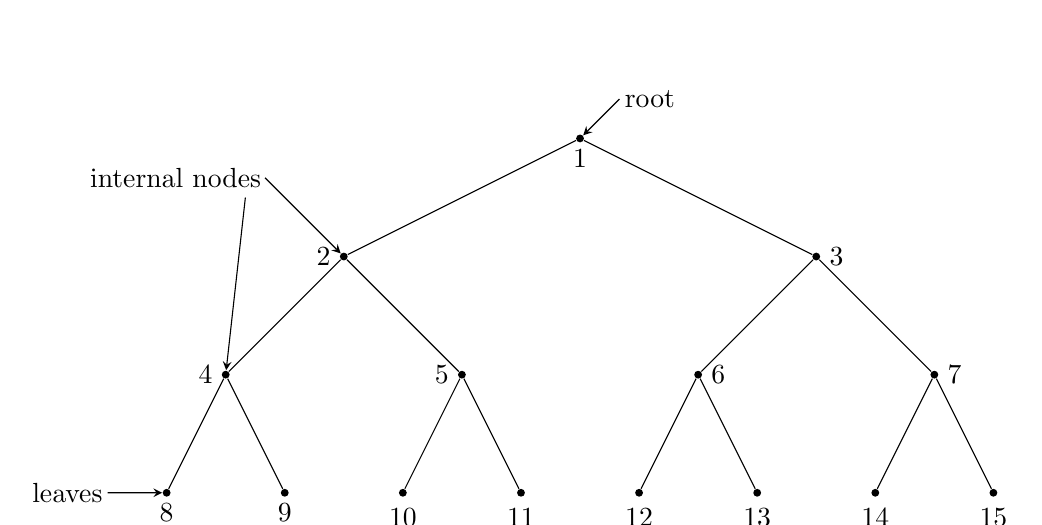
\begin{tikzpicture}
			\tikzset{
			every node/.style = {circle,inner sep=1pt,fill=black, minimum size=2pt}
		}
		\draw node [label=below:$1$] (a) {}
			child { node [label=left:$2$] (b) {}
				child {node [label=left:$4$] (c) {}
					child {node [label=below:$8$] (d) {}}
					child {node [label=below:$9$]{}}
				}
				child [missing]
				child {node [label=left:$5$]{}
					child {node [label=below:$10$]{}}
					child {node [label=below:$11$]{}}
				}
			}
			child [missing]
			child [missing]
			child [missing]
			child {node [label=right:$3$]{}
				child {node [label=right:$6$]{}
					child {node [label=below:$12$]{}}
					child {node [label=below:$13$]{}}
				}
				child [missing]
				child {node [label=right:$7$]{}
					child {node [label=below:$14$]{}}
					child {node [label=below:$15$]{}}
				}
			};
		\coordinate[label=right:root](root) at (0.5, 0.5);
		\coordinate[label=left:internal nodes] (internalnodes) at (-4,-0.5);
		\coordinate (internalnodes2) at (-4.25,-0.75);
		\coordinate [label=left:leaves] (leaf) at (-6,-4.5);
		\draw [-stealth] (root) -- (a);
		\draw [-stealth] (internalnodes) -- (b);
		\draw [-stealth] (internalnodes2) -- (c);
		\draw [-stealth] (leaf) -- (d);
		\end{tikzpicture}
	\end{center}
	\captionof{figure}{A diagram of a (rooted) tree.}
\end{example}

If we have done computer science, we'll know that trees are ubiquitous in the field, serving as a good way to visualise problems. For example, we see it appear in tree recursion.

Later on in this chapter, we will revisit the concept of trees and discuss it further.

\subsection{Planar Graphs}
\begin{defn}[Planar Graphs]
	A graph is planar if it can be drawn on the plane without crossings.
\end{defn}

What is important to note about planar graphs here is that, if there is a way to draw a graph without any crossings, if we then move the line so that there will be a crossing, it doesn't make the graph become non-planar.

We will introduce a few examples below in order to help visualise the idea of (non-)planar graphs better.

\begin{example}
	Below are examples of planar and non-planar graphs:
	\begin{center}
		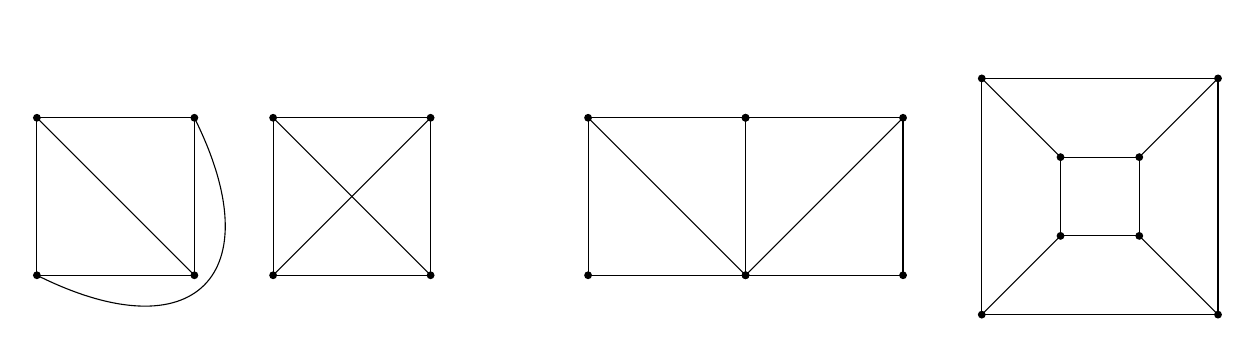
\begin{tikzpicture}
			\begin{scope}
				\coordinate (1) at (0,0);
				\coordinate (2) at (2,0);
				\coordinate (3) at (2,2);
				\coordinate (4) at (0,2);
				\node at (1) {};
				\node at (2) {};
				\node at (3) {};
				\node at (4) {};
				\draw (1) -- (2) -- (3) -- (4) -- (1);
				\draw (2) -- (4);
				\draw (0,0) .. controls (2,-1) and (3,0) .. (2,2);
				\foreach \Nombre in {1,2,3,4}
				\node[circle,inner sep=1pt,fill=black] at (\Nombre) {};
			\end{scope}
			\begin{scope}[shift={(3,0)}]
				\coordinate (1) at (0,0);
				\coordinate (2) at (2,0);
				\coordinate (3) at (2,2);
				\coordinate (4) at (0,2);
				\node at (1) {};
				\node at (2) {};
				\node at (3) {};
				\node at (4) {};
				\draw (1) -- (2) -- (3) -- (4) -- (1);
				\draw (2) -- (4);
				\draw (1) -- (3);
				\foreach \Nombre in {1,2,3,4}
				\node[circle,inner sep=1pt,fill=black] at (\Nombre) {};
			\end{scope}
			\begin{scope}[shift={(7,0)}]
				\coordinate (1) at (0,0);
				\coordinate (2) at (2,0);
				\coordinate (3) at (2,2);
				\coordinate (4) at (0,2);
				\node at (1) {};
				\node at (2) {};
				\node at (3) {};
				\node at (4) {};
				\draw (1) -- (2) -- (3) -- (4) -- (1);
				\draw (2) -- (4);
				\foreach \Nombre in {1,2,3,4}
				\node[circle,inner sep=1pt,fill=black] at (\Nombre) {};
			\end{scope}
			\begin{scope}[shift={(9,0)}]
				\coordinate (1) at (0,0);
				\coordinate (2) at (2,0);
				\coordinate (3) at (2,2);
				\coordinate (4) at (0,2);
				\node at (1) {};
				\node at (2) {};
				\node at (3) {};
				\node at (4) {};
				\draw (1) -- (2) -- (3) -- (4) -- (1);
				\draw (1) -- (3);
				\foreach \Nombre in {1,2,3,4}
				\node[circle,inner sep=1pt,fill=black] at (\Nombre) {};
			\end{scope}
			\begin{scope}[shift={(12,-0.5)}]
				\coordinate (1) at (0,0);
				\coordinate (2) at (3,0);
				\coordinate (3) at (3,3);
				\coordinate (4) at (0,3);
				\coordinate (5) at (1, 1);
				\coordinate (6) at (2, 1);
				\coordinate (7) at (2, 2);
				\coordinate (8) at (1, 2);
				\node at (1) {};
				\node at (2) {};
				\node at (3) {};
				\node at (4) {};
				\node at (5) {};
				\node at (6) {};
				\node at (7) {};
				\node at (8) {};
				\draw (1) -- (2) -- (3) -- (4) -- (1);
				\draw (5) -- (6) -- (7) -- (8) -- (5);
				\draw (1) -- (5);
				\draw (2) -- (6);
				\draw (3) -- (7);
				\draw (4) -- (8);
				\foreach \Nombre in {1,2,3,4,5,6,7,8}
				\node[circle,inner sep=1pt,fill=black] at (\Nombre) {};
			\end{scope}
		\end{tikzpicture}
	\end{center}
	\captionof{figure}{Example of various planar graphs.}
	
	We see that even though the second graph has crossings, as we can draw it without crossing, it is still considered planar. 
	
	Below are examples of non-planar graphs:
	
	\begin{center}
		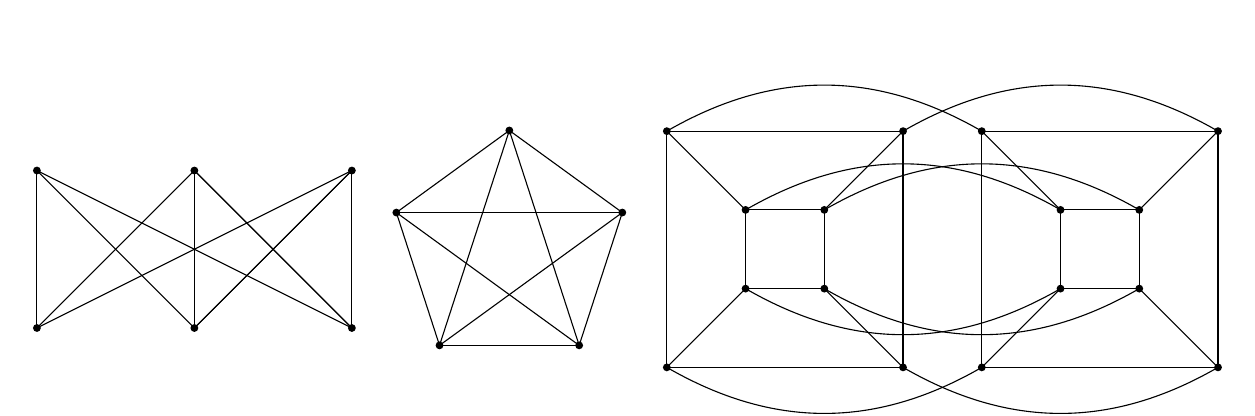
\begin{tikzpicture}
			\begin{scope}
				\coordinate (1) at (0,0);
				\coordinate (2) at (2,0);
				\coordinate (3) at (2,2);
				\coordinate (4) at (0,2);
				\coordinate (6) at (4,2);
				\coordinate (5) at (4,0);
				\node at (1) {};
				\node at (2) {};
				\node at (3) {};
				\node at (4) {};
				\node at (5) {};
				\node at (6) {};
				\draw (1) -- (4);
				\draw (2) -- (3);
				\draw (5) -- (6);
				\draw (1) -- (3);
				\draw (2) -- (4);
				\draw (2) -- (6);
				\draw (3) -- (5);
				\draw (1) -- (6);
				\draw (2) -- (6);
				\draw (5) -- (4);
				\draw (3) -- (5);
				\foreach \Nombre in {1,2,3,4,5,6}
				\node[circle,inner sep=1pt,fill=black] at (\Nombre) {};
			\end{scope}
			\begin{scope}[shift={(6,1)}]
				\node[
				regular polygon,
				regular polygon sides=5,
				minimum width=30mm,
				] (PG) {}
				(PG.corner 1) coordinate (PG1) {}
				(PG.corner 2) coordinate (PG2) {}
				(PG.corner 3) coordinate (PG3) {}
				(PG.corner 4) coordinate (PG4) {}
				(PG.corner 5) coordinate (PG5) {}
				;
				\foreach \S in {1,2,3,4,5}{
					\node at (PG\S) {};
				}
				\foreach \S/\E in {
					1/3, 1/4, 1/5,
					2/1, 2/3, 2/4, 2/5,
					3/4,
					5/3, 5/4%
				} {
					\draw (PG\S) -- (PG\E);
				}
				\foreach \Nombre in {PG1, PG2, PG3, PG4, PG5}
					\node[circle,inner sep=1pt,fill=black] at (\Nombre) {};
			\end{scope}
			\begin{scope}[shift={(8,-0.5)}]
				\coordinate (1) at (0,0);
				\coordinate (2) at (3,0);
				\coordinate (3) at (3,3);
				\coordinate (4) at (0,3);
				\coordinate (5) at (1, 1);
				\coordinate (6) at (2, 1);
				\coordinate (7) at (2, 2);
				\coordinate (8) at (1, 2);
				%
				\coordinate (9) at (4,0);
				\coordinate (10) at (7,0);
				\coordinate (11) at (7,3);
				\coordinate (12) at (4,3);
				\coordinate (13) at (5, 1);
				\coordinate (14) at (6, 1);
				\coordinate (15) at (6, 2);
				\coordinate (16) at (5, 2);
				\node at (9) {};
				\node at (10) {};
				\node at (11) {};
				\node at (12) {};
				\node at (13) {};
				\node at (14) {};
				\node at (15) {};
				\node at (16) {};
				\draw (1) -- (2) -- (3) -- (4) -- (1);
				\draw (5) -- (6) -- (7) -- (8) -- (5);
				\draw (1) -- (5);
				\draw (2) -- (6);
				\draw (3) -- (7);
				\draw (4) -- (8);
				\draw (9) -- (10) -- (11) -- (12) -- (9);
				\draw (13) -- (14) -- (15) -- (16) -- (13);
				\draw (9) -- (13);
				\draw (10) -- (14);
				\draw (11) -- (15);
				\draw (12) -- (16);
				\foreach \S/\E in{1/9, 2/10, 5/13, 6/14}
					\path (\S) edge [bend right] (\E);
				\foreach \S/\E in{3/11, 4/12, 7/15, 8/16}
				\path (\S) edge [bend left] (\E);
				\foreach \Nombre in {1,2,3,4,5,6,7,8,9,10,11,12,13,14,15,16}
					\node[circle,inner sep=1pt,fill=black] at (\Nombre) {};
			\end{scope}
		\end{tikzpicture}
	\end{center}
	\captionof{figure}{Example of various non-planar graphs.}
	
	We see that the three graphs above are non-planar. 
	
	\begin{enumerate}
		\item The first one is actually the infamous ``three house-three wells graph," also called $K_{3,3}$. The notation tells us that there are two sets of vertices, each of size three and all edges between the two sets of vertices are present.
	
		\item The second graph is the ``complete" graph with five nodes, or $K_{5}$.
	
		\item The third graph is a four-dimensional cube.
	\end{enumerate}
\end{example}

\begin{defn}[Bipartite Graphs]
	A useful concept is the notion of a bipartite graph, $G=(V,E)$, which is a graph where the vertices are split into two groups and edges only go between groups.
	
	More formally, we have $V = L \cup R$, and $E \subseteq L \times R$.
\end{defn}

From Example 4.25, we see that both $K_{3,3}$ and the hypercube are both bipartite. The latter follows from the fact that every cycle in the cube has an even length; this equivalence will be shown later in this chapter.

Now, when a planar graph is drawn on the plane, other than the number of vertices $v$ and edges $e$, we can distinguish between them by the number of faces $f$ that they have. The faces are the regions into which the graph subdivides the plane. For example, we see that the first graph has $4$ faces, while the third graph has $6$.

Now, we will introduce a key formula in regards to planar graphs:
\begin{thm}[Euler's formula]
	For every connected planar graph, $v + f = e + 2$
\end{thm}
\begin{proof}
	We shall proceed by induction on $e$, the number of edges of our planar graph $G$.
	
	\textbf{\underline{Base Case}}: We see that for $e=0$, $G$ has only one vertex and one face. Thus, $v+f=2$, and we see that our claim holds for our base case.
	
	\textbf{\underline{Induction Hypothesis}}: Suppose that for $e-1$ edges, our claim holds true. 
	
	\textbf{\underline{Inductive Step}}: Now, we want to prove that our induction hypothesis holds for a graph with $e$. First, we have two cases:
	\begin{enumerate}
		\item $G$ does not contain a cycle. Then, our planar graph is a tree. In this case then, by definition, we observe that the graph has $1$ face, and $e=v-1$. Then, we see the following:
		\begin{align*}
			v + f &= e + 2 \\
			v + 1 &= (v-1) + 2 \\
			&= v + 1
		\end{align*}
		Thus, we see that our claim holds true in this case.
		
		\item If our graph does contain a cycle, which we will denote as $C$, then we observe that by removing an edge $e'$ from $C$, we will reduce the number of faces by $1$. Let us call the new graph created by this action $G'$.
		
		We now observe that since $G'$ has $e-1$ edges, we can apply our induction hypothesis. That is, $v+(f-1)=(e-1)+2$. Then, from this, we observe that $v+f = e+2$.
	\end{enumerate}

	Thus, by mathematical induction, we can conclude that our claim is true.
\end{proof}

Now, what happens if the graph isn't connected? How do the number of connected components enter the formula?

Take a planar graph with $f$ faces, and consider one face. It has a number of sides --- that is, edges that bound it clockwise. Note that an edge may be counted twice, if it has the same face on both sides (such as in trees).

Now, denote the number of sides of face $i$ by $s_{i}$. If we add the $s_{i}$'s together, we will get $2e$, as each edge is counted twice: once for the face on its right, and once for the face on its left (they may coincide if the edge is a bridge). This observation yields us the following:
\begin{thm}
	For any planar graph, we have
	\begin{equation*}
		\sum{i=1}{f} s_{i} = 2e
	\end{equation*}
\end{thm}

Now, notice that as we don't allow for parallel edges between the same two nodes and if we assume that there are at least two edges (meaning, there are at least three vertices), then every face has at least three sides. In other words, $s_{i} \geq 3$ for all $i$. Then, it follows that $3f \leq 2e$. Using Euler's formula, we observe the following:
\begin{equation*}
	e \leq 	3v - 6
\end{equation*}

What this inequality tells us is that planar graphs are sparse; they can't have too many edges.
\begin{example}
	For example, consider a 1000-vertex connected graph. We see that it can have anywhere from 1000 to 500000 edges. Meanwhile, we see that for planar graphs, the range is small: between 999 and 2994.
\end{example}

Now, the inequality also tells us that $K_{5}$ is not a planar graph; it has 10 edges, but only 5 vertices; $10 \not\leq 9$.

Now, observe that for $K_{3,3}$, it has 9 edges and 6 vertices; $9 \leq 12$, so it is planar, right? Well, we have to think a bit harder about this graph. Below, we have $K_{3,3}$ with each node labeled clockwise.
\begin{center}
	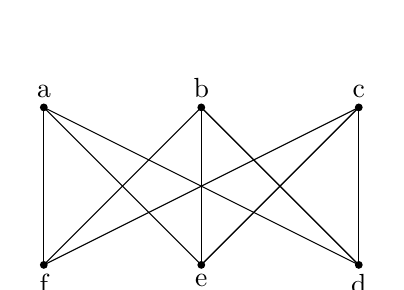
\begin{tikzpicture}
		\begin{scope}
			\coordinate [label=below:f](1) at (0,0);
			\coordinate [label=below:e](2) at (2,0);
			\coordinate [label=above:b](3) at (2,2);
			\coordinate [label=above:a](4) at (0,2);
			\coordinate [label=above:c](6) at (4,2);
			\coordinate [label=below:d](5) at (4,0);
			\node at (1) {};
			\node at (2) {};
			\node at (3) {};
			\node at (4) {};
			\node at (5) {};
			\node at (6) {};
			\draw (1) -- (4);
			\draw (2) -- (3);
			\draw (5) -- (6);
			\draw (1) -- (3);
			\draw (2) -- (4);
			\draw (2) -- (6);
			\draw (3) -- (5);
			\draw (1) -- (6);
			\draw (2) -- (6);
			\draw (5) -- (4);
			\draw (3) -- (5);
			\foreach \Nombre in {1,2,3,4,5,6}
			\node[circle,inner sep=1pt,fill=black] at (\Nombre) {};
		\end{scope}
	\end{tikzpicture}
\end{center}
\captionof{figure}{$K_{3,3}$ with its nodes labeled.}

Now, let us first remove the three vertical edges: $\left\{ (a,f), (b,e), (c,d) \right\}$. We shall call this graph $K'$.
\begin{center}
	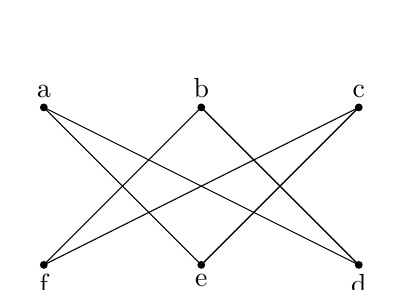
\begin{tikzpicture}
		\begin{scope}
			\coordinate [label=below:f](1) at (0,0);
			\coordinate [label=below:e](2) at (2,0);
			\coordinate [label=above:b](3) at (2,2);
			\coordinate [label=above:a](4) at (0,2);
			\coordinate [label=above:c](6) at (4,2);
			\coordinate [label=below:d](5) at (4,0);
			\node at (1) {};
			\node at (2) {};
			\node at (3) {};
			\node at (4) {};
			\node at (5) {};
			\node at (6) {};
			\draw (1) -- (3);
			\draw (2) -- (4);
			\draw (2) -- (6);
			\draw (3) -- (5);
			\draw (1) -- (6);
			\draw (2) -- (6);
			\draw (5) -- (4);
			\draw (3) -- (5);
			\foreach \Nombre in {1,2,3,4,5,6}
			\node[circle,inner sep=1pt,fill=black] at (\Nombre) {};
		\end{scope}
	\end{tikzpicture}
\end{center}
\captionof{figure}{A depiction of $K'$, which is $K_{3,3}$ with some edges removed.}

From here, we see that $K'$ is a six-vertex planar graph, depicted below, with two of the removed edges added back in using red:
\begin{center}
	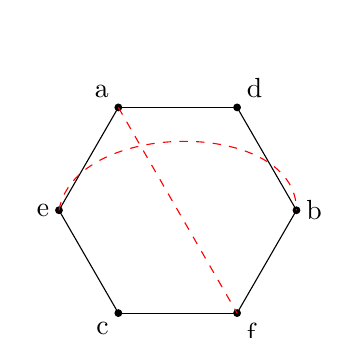
\begin{tikzpicture}
		\node[
		regular polygon,
		regular polygon sides=6,
		minimum width=30mm,
		] (PG) {}
		(PG.corner 1) coordinate[label=above right:d] (PG1) {}
		(PG.corner 2) coordinate[label=above left: a] (PG2) {}
		(PG.corner 3) coordinate[label=left: e] (PG3) {}
		(PG.corner 4) coordinate[label=below left: c] (PG4) {}
		(PG.corner 5) coordinate[label=below right: f] (PG5) {}
		(PG.corner 6) coordinate[label=right: b] (PG6) {}
		;
		\foreach \S in {1,2,3,4,5,6}{
			\node at (PG\S) {};
		}
		\foreach \A/\B in {1/2, 2/3, 3/4, 4/5, 5/6, 6/1}{
			\draw (PG\A) -- (PG\B);
		}
		\foreach \N in {1,2,3,4,5,6}{
			\node[circle,inner sep=1pt,fill=black] at (PG\N) {};
		}
		\draw[red][dashed] (PG2) -- (PG5);
		\draw[red][dashed] (PG3.north) to [out=80, in=90] (PG6.north);
	\end{tikzpicture}
\end{center}
\captionof{figure}{A depiction of $K'$ redrawn as a planar graph, along with two edges added back in.}

From here, we see that it is impossible for us to have the removed edges be added back in without intersection. As such, we can conclude that $K_{3,3}$ must be non-planar.

Now, from this, we uncover an interesting theorem:
\begin{thm}
	A graph is non-planar if and only if it contains $K_{5}$ or $K_{3,3}$.
\end{thm}

Of course, one of the direction is very straightforward to prove: we observe that if a graph $G$ contains $K_{5}$ or $K_{3,3}$, then as these graphs are non-planar, $G$ must be non-planar as well.

The other direction, however, is harder to prove... and will be left as an exercise for the future.

\section{Duality and Colouring}
\begin{defn}[Duality]
	Take a planar graph $G$, and assume that it has no bridges and no degree-two nodes. Now, draw a new graph $G*$ via the following steps:
	\begin{enumerate}
		\item Start by placing a node on each face of $G$.
		\item Draw an edge between two faces if they touch at an edge --- draw the new edge so that it crosses that edge.
	\end{enumerate}
	Now, the result is a planar graph $G*$. What is interesting is that the dual of $G*$ (that is, $(G*)*$) is the original graph, $G$.
\end{defn}

The idea of duality is a convenient way to look at planar graphs. It also tells us that ``colouring a political map so that no two countries sharing a border have the same colour" is the same problem as ``colouring the vertices of a planar graph (the dual of a political map) so that no two adjacent vertices have the same colour."

\subsection{Bipartite Graphs and Colouring}
We will briefly talk about bipartite graphs in the context of colouring. Observe that a two-colourable graph is equivalent to a bipartite graph as the colouring splits the vertices into two sets, where the edges only connect vertices in the two colours.

From this observation, we can see that a graph that doesn't have any odd length cycle is bipartite as we can colour any such graph using two colours. This is accomplished by doing the following:
\begin{itemize}
	\item Colour a vertex $x$ red. Then, colour its neighbour blue. We continue by colouring the next uncoloured neighbour red, then blue, and keep on alternating colours like this.
	
	\item Now, if this doesn't work then it means that there must be an edge connecting two vertices of the same colour. Let us denote this edge as $(u,v)$. Then, we can identify an odd cycle by using the path $p_{1}$ from $x$ to $u$ and $p_{2}$ from $v$ to $x$. We remove the common portions of $p_{1}$ and $p_{2}$. Notice that the length of the two paths have the same parity (they're either both even, or both odd) as $u$ and $v$ have the same colour. Then, the total length of the cycle must thus be odd as we include the extra edge $(u,v)$.
\end{itemize}

\subsection{The Five Colour Theorem}
One of the most famous theorems is the four colour theorem. For this subsection, we will prove a weaker version of it:
\begin{thm}[Five Colour Theorem]
	Every planar graph can be coloured with five colours.
\end{thm}
\begin{proof}
	We shall proceed by induction on $v$, where $v$ is the vertices of a planar graph $G$.
	
	Before we start with our induction proof, we first observe that for any valid colouring of a graph, we can swap the colours for each pair of vertices 
\end{proof}


\chapter{Modular Arithmetic}
\section{Modular Arithmetic}
An intuitive way of thinking about modular arithmetic is about our clock system. Say we are using a 24-hour clock system, and we're at 23:00. If we add 8 hours, we'd get $(23+8=)$ 31:00.

However, this isn't the correct time as we are on a 24-hour system. Instead, it ``wraps" around 00:00, and becomes $(31-24=)$ 7:00.

In modular arithmetic, we perform arithmetic operations relative to a fixed $n$ called the modulus. For our 24-hour clock system, $n=24$. In the example given, we can rewrite it as:

\begin{equation*}
	31\Mod{24}=7
\end{equation*}

The function ``$\Mod{24}$" returns the remainder we get when dividing by 24.

\subsection{Addition, Subtraction, Multiplication}
One of the properties of numbers modulo $n$ is the arithmetic operations we are familiar with. First, we will start out with addition.

Say we want to find $42+35\Mod{24}$. We have two ways of doing so:
\begin{enumerate}
	\item $42+35\Mod{24}=77\Mod{24}=5$
	\item $42+35\Mod{24}=[42\Mod{24}]+[35\Mod{24}]\Mod{24}=18+11\Mod{24}=29\Mod{24}=5$
\end{enumerate}

Regardless of the sequence in which we perform arithmetic operations $\Mod{24}$, we will still get the same result; we can reduce $\Mod{24}$ only once at the end, or reduce each or even just some intermediate result $\Mod{24}$ (as long as we reduce the final answer $\Mod{24}$. To see why this is, we have to view numbers modulo $n$ in a different way.

For two integers $a$ and $b$, we say $a$ is congruent to $b$ modulo $n$ iff $a\Mod{n}=b\Mod{n}$. We write this as:
\begin{equation*}
	a\equiv_nb\iff n|(a-b)
\end{equation*}

In other words, $a$ and $b$ have the same remainder when we divide them by $n$. From this, we see that using $a$ or $b$ in arithmetic operations will yield the same result.

Also, note that $p|q$ means $p$ divides $q$; in other words, $\frac{q}{p}$ returns an integer. Equivalently, we can say that for $k\in\mathbb{Z}$:
\begin{equation*}
	a=b+kn
\end{equation*}

So, for $n=24$ we see all of these numbers are congruent to each other:
\begin{align*}
	\ldots\equiv_{24}-24\equiv_{24}0\equiv_{24}24\equiv_{24}\ldots \\
	\ldots\equiv_{24}-23\equiv_{24}1\equiv_{24}25\equiv_{24}\ldots
\end{align*}

And there are 24 such disjoint sets where all of the numbers in each set are congruent to one another. 

In general, if we work modulo $n$, then we get $n$ disjoint sets such that the union of these sets forms the set of all integers: these are often called \textit{residue classes mod n}.

There are $n$ residue classes, which are represented by a number $i\in\{0,\ldots,n-1\}$. And the elements in a set represented by the residue $i$ are simply $m=i+kn$, where $k\in\mathbb{Z}$.

Now, we will introduce the following theorem:
\begin{theorem}
	For all $n \geq 1$ and $a,b,c,d\in\mathbb{Z}$, the following are true:
	\begin{enumerate}
		\item If $a \equiv_n b$ and $c \equiv_n d$, then $a+c \equiv_n b+d$
		\item If $a \equiv_n b$ and $c \equiv_n d$, then $a \cdot c \equiv_n b \cdot d$
	\end{enumerate}
\end{theorem}
\begin{proof}
	We will proceed to prove the theorem above. Recall that since $a \equiv_n b$, then that means that there's a $k\in\mathbb{Z}$ such that $a=b+kn$. Similarly, $c=d+\ell n$ for $\ell\in\mathbb{Z}$.
	
	Now, we will begin with the first part of the theorem:
	
	\begin{align*}
		a+c&=(b+kn)+(d+\ell n) \\
		&=(b+d)+(kn+\ell n) \\
		&=(b+d)+(k+\ell)n
	\end{align*}
	
	And notice here that since $k$ and $\ell$ are both integers, then $k \ell$ is also an integer. Thus, we can rewrite the equation as the following:
	
	\begin{equation*}
		a+c=(b+d)+mn, \quad m\in\mathbb{Z}
	\end{equation*}
	
	From this, we can see that $a+c \equiv_n b+d$; we have proven the first part of the theorem. Now, for the second part of the theorem:
	
	\begin{align*}
		a \cdot c&=(b+kn)(d+\ell n) \\
		&=bd + \ell bn + kdn + k\ell n^2 \\
		&= bd + (\ell b + kd + k\ell n)n
	\end{align*}
	
	Similarly, we see here that since $b,d,k,\ell\in\mathbb{Z}$, then $(\ell b + kd + k\ell n)\in\mathbb{Z}$. As such, we can rewrite the equation as:
	
	\begin{equation*}
		a \cdot c = bd + mn, \quad m\in\mathbb{Z}
	\end{equation*}
	
	From this, we can see that $a \cdot c \equiv_n b \cdot d$, and thus the second part of the theorem has been proven; and, with both parts proven, we've proven the theorem.
\end{proof}

\subsection{Exponentiation}
Another standard operation in arithmetic algorithms is raising a number to a power modulo another number; in other words, how can we compute $x^y\Mod{m}$, where $x,y,m\in\mathbb{N}$, and $m>0$?

For small numbers of $x,y$, it may seem redundant

\subsection{Division and Multiplicative Inverse}
In Section 1.1, we discuss addition/subtraction/multiplication in  the setting of modular arithmetic. However, division is a little bit more tricky to work with, hence why this subsection will be dedicated to it alone.

First, we will look at division done over rational numbers $\mathbb{Q}$. Here, if we want to divide $x\in\mathbb{Q}$ by $y\in\mathbb{Q}$

\end{document}
